% Options for packages loaded elsewhere
% Options for packages loaded elsewhere
\PassOptionsToPackage{unicode}{hyperref}
\PassOptionsToPackage{hyphens}{url}
\PassOptionsToPackage{dvipsnames,svgnames,x11names}{xcolor}
%
\documentclass[
  brazilian,
  letterpaper,
  DIV=11,
  numbers=noendperiod]{scrreprt}
\usepackage{xcolor}
\usepackage{amsmath,amssymb}
\setcounter{secnumdepth}{5}
\usepackage{iftex}
\ifPDFTeX
  \usepackage[T1]{fontenc}
  \usepackage[utf8]{inputenc}
  \usepackage{textcomp} % provide euro and other symbols
\else % if luatex or xetex
  \usepackage{unicode-math} % this also loads fontspec
  \defaultfontfeatures{Scale=MatchLowercase}
  \defaultfontfeatures[\rmfamily]{Ligatures=TeX,Scale=1}
\fi
\usepackage{lmodern}
\ifPDFTeX\else
  % xetex/luatex font selection
\fi
% Use upquote if available, for straight quotes in verbatim environments
\IfFileExists{upquote.sty}{\usepackage{upquote}}{}
\IfFileExists{microtype.sty}{% use microtype if available
  \usepackage[]{microtype}
  \UseMicrotypeSet[protrusion]{basicmath} % disable protrusion for tt fonts
}{}
\makeatletter
\@ifundefined{KOMAClassName}{% if non-KOMA class
  \IfFileExists{parskip.sty}{%
    \usepackage{parskip}
  }{% else
    \setlength{\parindent}{0pt}
    \setlength{\parskip}{6pt plus 2pt minus 1pt}}
}{% if KOMA class
  \KOMAoptions{parskip=half}}
\makeatother
% Make \paragraph and \subparagraph free-standing
\makeatletter
\ifx\paragraph\undefined\else
  \let\oldparagraph\paragraph
  \renewcommand{\paragraph}{
    \@ifstar
      \xxxParagraphStar
      \xxxParagraphNoStar
  }
  \newcommand{\xxxParagraphStar}[1]{\oldparagraph*{#1}\mbox{}}
  \newcommand{\xxxParagraphNoStar}[1]{\oldparagraph{#1}\mbox{}}
\fi
\ifx\subparagraph\undefined\else
  \let\oldsubparagraph\subparagraph
  \renewcommand{\subparagraph}{
    \@ifstar
      \xxxSubParagraphStar
      \xxxSubParagraphNoStar
  }
  \newcommand{\xxxSubParagraphStar}[1]{\oldsubparagraph*{#1}\mbox{}}
  \newcommand{\xxxSubParagraphNoStar}[1]{\oldsubparagraph{#1}\mbox{}}
\fi
\makeatother

\usepackage{color}
\usepackage{fancyvrb}
\newcommand{\VerbBar}{|}
\newcommand{\VERB}{\Verb[commandchars=\\\{\}]}
\DefineVerbatimEnvironment{Highlighting}{Verbatim}{commandchars=\\\{\}}
% Add ',fontsize=\small' for more characters per line
\usepackage{framed}
\definecolor{shadecolor}{RGB}{241,243,245}
\newenvironment{Shaded}{\begin{snugshade}}{\end{snugshade}}
\newcommand{\AlertTok}[1]{\textcolor[rgb]{0.68,0.00,0.00}{#1}}
\newcommand{\AnnotationTok}[1]{\textcolor[rgb]{0.37,0.37,0.37}{#1}}
\newcommand{\AttributeTok}[1]{\textcolor[rgb]{0.40,0.45,0.13}{#1}}
\newcommand{\BaseNTok}[1]{\textcolor[rgb]{0.68,0.00,0.00}{#1}}
\newcommand{\BuiltInTok}[1]{\textcolor[rgb]{0.00,0.23,0.31}{#1}}
\newcommand{\CharTok}[1]{\textcolor[rgb]{0.13,0.47,0.30}{#1}}
\newcommand{\CommentTok}[1]{\textcolor[rgb]{0.37,0.37,0.37}{#1}}
\newcommand{\CommentVarTok}[1]{\textcolor[rgb]{0.37,0.37,0.37}{\textit{#1}}}
\newcommand{\ConstantTok}[1]{\textcolor[rgb]{0.56,0.35,0.01}{#1}}
\newcommand{\ControlFlowTok}[1]{\textcolor[rgb]{0.00,0.23,0.31}{\textbf{#1}}}
\newcommand{\DataTypeTok}[1]{\textcolor[rgb]{0.68,0.00,0.00}{#1}}
\newcommand{\DecValTok}[1]{\textcolor[rgb]{0.68,0.00,0.00}{#1}}
\newcommand{\DocumentationTok}[1]{\textcolor[rgb]{0.37,0.37,0.37}{\textit{#1}}}
\newcommand{\ErrorTok}[1]{\textcolor[rgb]{0.68,0.00,0.00}{#1}}
\newcommand{\ExtensionTok}[1]{\textcolor[rgb]{0.00,0.23,0.31}{#1}}
\newcommand{\FloatTok}[1]{\textcolor[rgb]{0.68,0.00,0.00}{#1}}
\newcommand{\FunctionTok}[1]{\textcolor[rgb]{0.28,0.35,0.67}{#1}}
\newcommand{\ImportTok}[1]{\textcolor[rgb]{0.00,0.46,0.62}{#1}}
\newcommand{\InformationTok}[1]{\textcolor[rgb]{0.37,0.37,0.37}{#1}}
\newcommand{\KeywordTok}[1]{\textcolor[rgb]{0.00,0.23,0.31}{\textbf{#1}}}
\newcommand{\NormalTok}[1]{\textcolor[rgb]{0.00,0.23,0.31}{#1}}
\newcommand{\OperatorTok}[1]{\textcolor[rgb]{0.37,0.37,0.37}{#1}}
\newcommand{\OtherTok}[1]{\textcolor[rgb]{0.00,0.23,0.31}{#1}}
\newcommand{\PreprocessorTok}[1]{\textcolor[rgb]{0.68,0.00,0.00}{#1}}
\newcommand{\RegionMarkerTok}[1]{\textcolor[rgb]{0.00,0.23,0.31}{#1}}
\newcommand{\SpecialCharTok}[1]{\textcolor[rgb]{0.37,0.37,0.37}{#1}}
\newcommand{\SpecialStringTok}[1]{\textcolor[rgb]{0.13,0.47,0.30}{#1}}
\newcommand{\StringTok}[1]{\textcolor[rgb]{0.13,0.47,0.30}{#1}}
\newcommand{\VariableTok}[1]{\textcolor[rgb]{0.07,0.07,0.07}{#1}}
\newcommand{\VerbatimStringTok}[1]{\textcolor[rgb]{0.13,0.47,0.30}{#1}}
\newcommand{\WarningTok}[1]{\textcolor[rgb]{0.37,0.37,0.37}{\textit{#1}}}

\usepackage{longtable,booktabs,array}
\newcounter{none} % for unnumbered tables
\usepackage{calc} % for calculating minipage widths
% Correct order of tables after \paragraph or \subparagraph
\usepackage{etoolbox}
\makeatletter
\patchcmd\longtable{\par}{\if@noskipsec\mbox{}\fi\par}{}{}
\makeatother
% Allow footnotes in longtable head/foot
\IfFileExists{footnotehyper.sty}{\usepackage{footnotehyper}}{\usepackage{footnote}}
\makesavenoteenv{longtable}
\usepackage{graphicx}
\makeatletter
\newsavebox\pandoc@box
\newcommand*\pandocbounded[1]{% scales image to fit in text height/width
  \sbox\pandoc@box{#1}%
  \Gscale@div\@tempa{\textheight}{\dimexpr\ht\pandoc@box+\dp\pandoc@box\relax}%
  \Gscale@div\@tempb{\linewidth}{\wd\pandoc@box}%
  \ifdim\@tempb\p@<\@tempa\p@\let\@tempa\@tempb\fi% select the smaller of both
  \ifdim\@tempa\p@<\p@\scalebox{\@tempa}{\usebox\pandoc@box}%
  \else\usebox{\pandoc@box}%
  \fi%
}
% Set default figure placement to htbp
\def\fps@figure{htbp}
\makeatother



\ifLuaTeX
\usepackage[bidi=basic,shorthands=off]{babel}
\else
\usepackage[bidi=default,shorthands=off]{babel}
\fi
\ifLuaTeX
  \usepackage{selnolig} % disable illegal ligatures
\fi


\setlength{\emergencystretch}{3em} % prevent overfull lines

\providecommand{\tightlist}{%
  \setlength{\itemsep}{0pt}\setlength{\parskip}{0pt}}



 


\usepackage{fvextra}
\DefineVerbatimEnvironment{Highlighting}{Verbatim}{breaklines,commandchars=\\\{\}}
\KOMAoption{captions}{tableheading}
\makeatletter
\@ifpackageloaded{tcolorbox}{}{\usepackage[skins,breakable]{tcolorbox}}
\@ifpackageloaded{fontawesome5}{}{\usepackage{fontawesome5}}
\definecolor{quarto-callout-color}{HTML}{909090}
\definecolor{quarto-callout-note-color}{HTML}{0758E5}
\definecolor{quarto-callout-important-color}{HTML}{CC1914}
\definecolor{quarto-callout-warning-color}{HTML}{EB9113}
\definecolor{quarto-callout-tip-color}{HTML}{00A047}
\definecolor{quarto-callout-caution-color}{HTML}{FC5300}
\definecolor{quarto-callout-color-frame}{HTML}{acacac}
\definecolor{quarto-callout-note-color-frame}{HTML}{4582ec}
\definecolor{quarto-callout-important-color-frame}{HTML}{d9534f}
\definecolor{quarto-callout-warning-color-frame}{HTML}{f0ad4e}
\definecolor{quarto-callout-tip-color-frame}{HTML}{02b875}
\definecolor{quarto-callout-caution-color-frame}{HTML}{fd7e14}
\makeatother
\makeatletter
\@ifpackageloaded{bookmark}{}{\usepackage{bookmark}}
\makeatother
\makeatletter
\@ifpackageloaded{caption}{}{\usepackage{caption}}
\AtBeginDocument{%
\ifdefined\contentsname
  \renewcommand*\contentsname{Índice}
\else
  \newcommand\contentsname{Índice}
\fi
\ifdefined\listfigurename
  \renewcommand*\listfigurename{Lista de Figuras}
\else
  \newcommand\listfigurename{Lista de Figuras}
\fi
\ifdefined\listtablename
  \renewcommand*\listtablename{Lista de Tabelas}
\else
  \newcommand\listtablename{Lista de Tabelas}
\fi
\ifdefined\figurename
  \renewcommand*\figurename{Figura}
\else
  \newcommand\figurename{Figura}
\fi
\ifdefined\tablename
  \renewcommand*\tablename{Tabela}
\else
  \newcommand\tablename{Tabela}
\fi
}
\@ifpackageloaded{float}{}{\usepackage{float}}
\floatstyle{ruled}
\@ifundefined{c@chapter}{\newfloat{codelisting}{h}{lop}}{\newfloat{codelisting}{h}{lop}[chapter]}
\floatname{codelisting}{Listagem}
\newcommand*\listoflistings{\listof{codelisting}{Lista de Listagens}}
\makeatother
\makeatletter
\makeatother
\makeatletter
\@ifpackageloaded{caption}{}{\usepackage{caption}}
\@ifpackageloaded{subcaption}{}{\usepackage{subcaption}}
\makeatother
\usepackage{bookmark}
\IfFileExists{xurl.sty}{\usepackage{xurl}}{} % add URL line breaks if available
\urlstyle{same}
% fallback for those not using the hyperref driver hyperxmp:
\makeatletter
\@ifundefined{xmpquote}{\newcommand{\xmpquote}[1]{#1}}{}
\makeatother
\hypersetup{
  pdftitle={Treinamento em Nextflow},
  pdflang={pt-BR},
  colorlinks=true,
  linkcolor={blue},
  filecolor={Maroon},
  citecolor={Blue},
  urlcolor={Blue},
  pdfcreator={LaTeX via pandoc}}


\title{Treinamento em Nextflow}
\author{}
\date{}
\begin{document}
\maketitle

\RecustomVerbatimEnvironment{verbatim}{Verbatim}{
  showspaces = false,
  showtabs = false,
  breaksymbolleft={},
  breaklines
  % Note: setting commandchars=\\\{\} here will cause an error 
}

\renewcommand*\contentsname{Índice}
{
\setcounter{tocdepth}{2}
\tableofcontents
}

\bookmarksetup{startatroot}

\chapter{Treinamento Nextflow}\label{treinamento-nextflow}

\section{Visão geral do curso}\label{visuxe3o-geral-do-curso}

Este curso é divido em duas partes, no primeiro momento veremos como o
nextflow é estruturado e no segundo momento aprenderemos a executar e
personalizar pipelines já existentes. Cada sessão possui objetivos
estruturados para introduzir informações gradualmente.

\bookmarksetup{startatroot}

\chapter{Ambiente de trabalho}\label{ambiente-de-trabalho}

\section{Ambiente Local}\label{ambiente-local}

Caso todas as dependencias necessárias para execução desse minicurso
estejam instaladas em sua máquina local, clone o repositório deste
minicurso:

\begin{Shaded}
\begin{Highlighting}[]
\FunctionTok{git}\NormalTok{ clone git@github.com:dalmolingroup/nextflow\_training.git}

\BuiltInTok{cd}\NormalTok{ nextflow\_training}
\end{Highlighting}
\end{Shaded}

\section{Ambiente Remoto}\label{ambiente-remoto}

Caso não as dependencias necessárias para este minicurso não estejam
instaladas na sua máquina local, você poderá utilizar o ambiente
pré-construído fornecido pela Seqera no
\href{https://codespaces.new/nextflow-io/training?quickstart=1&ref=3.6.1}{GitHub
Codespace}. Este ambiente de treinamento contém todo o software, código
e dados necessários para trabalhar no curso de treinamento, então você
não precisa instalar nada por conta própria.

\bookmarksetup{startatroot}

\chapter{Objetivos}\label{objetivos}

Ao final do minicurso, você deverá ser capaz de:

\begin{itemize}
\tightlist
\item
  Entender a estrutura básica de um pipeline Nextflow (processos,
  canais, workflow, módulos)
\item
  Executar pipelines nf-core prontos usando perfis de teste
\item
  Configurar a execução via \texttt{params}, \texttt{-params-file} e
  arquivos de configuração
\item
  Personalizar recursos e argumentos de ferramentas usando
  \texttt{ext.args}
\item
  Instalar e usar módulos do repositório nf-core
\item
  Diagnosticar erros comuns a partir das mensagens de validação de
  schema/samplesheet
\end{itemize}

\section{\texorpdfstring{O que este curso \textbf{não}
cobre}{O que este curso não cobre}}\label{o-que-este-curso-nuxe3o-cobre}

\begin{itemize}
\tightlist
\item
  Programação em Nextflow do zero (não vamos escrever pipelines novos)
\item
  Operadores avançados de canais (\texttt{flatten}, \texttt{groupTuple},
  \texttt{join}, etc.)
\item
  Desenvolvimento de módulos nf-core seguindo o template completo
\item
  Criação de subworkflows
\end{itemize}

\bookmarksetup{startatroot}

\chapter{Pré-requisitos:}\label{pruxe9-requisitos}

\begin{itemize}
\tightlist
\item
  Confortável com o terminal Linux (\texttt{cd}, \texttt{ls}, editar
  arquivos)
\item
  Docker instalado e funcional (ou usar o ambiente remoto via GitHub
  Codespaces)
\item
  Nextflow instalado (ou usar o ambiente remoto)
\item
  \texttt{nf-core\ tools} (para a parte de módulos)
\end{itemize}

\bookmarksetup{startatroot}

\chapter{Agenda (5h)}\label{agenda-5h}

{\def\LTcaptype{none} % do not increment counter
\begin{longtable}[]{@{}
  >{\raggedright\arraybackslash}p{(\linewidth - 4\tabcolsep) * \real{0.3333}}
  >{\raggedright\arraybackslash}p{(\linewidth - 4\tabcolsep) * \real{0.3333}}
  >{\raggedright\arraybackslash}p{(\linewidth - 4\tabcolsep) * \real{0.3333}}@{}}
\toprule\noalign{}
\begin{minipage}[b]{\linewidth}\raggedright
Bloco
\end{minipage} & \begin{minipage}[b]{\linewidth}\raggedright
Duração
\end{minipage} & \begin{minipage}[b]{\linewidth}\raggedright
Conteúdo
\end{minipage} \\
\midrule\noalign{}
\endhead
\bottomrule\noalign{}
\endlastfoot
\textbf{1. Hello Nextflow --- parte 1} & 45 min & História, estrutura de
pipeline, primeiro \texttt{hello-world.nf}, \texttt{.command.*},
\texttt{-resume}, \texttt{nextflow\ log} \\
\textbf{2. Hello Nextflow --- parte 2} & 45 min & Canais, workflow
multi-etapa, módulos, contêineres \\
\textbf{Intervalo} & 15 min & \\
\textbf{3. Configuração Nextflow} & 45 min & \texttt{nextflow.config},
diretivas de processo, profiles, \texttt{-params-file}, precedência \\
\textbf{4. Hello nf-core --- parte 1} & 60 min & O que é nf-core,
\texttt{nextflow\ pull}, perfil test, \texttt{-\/-help},
\texttt{-params-file}, \texttt{-c}, \texttt{ext.args} \\
\textbf{Intervalo} & 15 min & \\
\textbf{5. Validação de entrada} & 30 min & Schema de parâmetros, schema
de samplesheet, debug de erros \\
\textbf{6. Usando módulos nf-core} & 30 min & Catálogo,
\texttt{nf-core\ modules\ install}, \texttt{ext.args} para
customização \\
\textbf{7. Q\&A + prática livre} & 15 min & \\
\end{longtable}
}

\part{Hello Nextflow}

\chapter{Hello Nextflow}\label{hello-nextflow-1}

\section{O que é Nextflow}\label{o-que-uxe9-nextflow}

Nextflow é uma linguagem de fluxo de trabalho (workflow language) criada
em 2013 pelo Paolo Di Tommaso no Centre for Genomic Regulation
(Barcelona), pensada para orquestrar pipelines científicos que envolvem
muitas ferramentas e muitos dados.

Hoje é mantido pela \textbf{Seqera Labs} (a empresa fundada por Paolo)
junto com uma comunidade global de contribuidores. A Seqera desenvolve o
Nextflow como open source e oferece produtos comerciais em cima dele
(Seqera Platform, Wave, Fusion), mas o Nextflow em si é livre.

\section{O ecossistema nf-core}\label{o-ecossistema-nf-core}

\textbf{nf-core} é uma comunidade independente que constrói pipelines
Nextflow curados, revisados por pares e testados --- hoje já são mais de
100 pipelines cobrindo genômica, transcriptômica, proteômica,
metagenômica etc. Todos seguem o mesmo template, o que significa que
aprender a rodar/customizar \textbf{um} pipeline nf-core te ensina a
rodar \textbf{todos}.

\section{Por que Nextflow}\label{por-que-nextflow}

\begin{itemize}
\tightlist
\item
  \textbf{Reprodutibilidade}: cada processo roda em um contêiner
  (Docker/Singularity/Conda). Você não precisa instalar dependências
  manualmente.
\item
  \textbf{Portabilidade}: o mesmo pipeline roda no seu laptop, num HPC
  (Slurm/PBS/SGE) ou na nuvem (AWS/Google/Azure), mudando só um perfil
  de configuração.
\item
  \textbf{\texttt{-resume}}: se um passo falha ou você muda um
  parâmetro, o Nextflow reaproveita tudo que já rodou. Fundamental para
  pipelines longos.
\item
  \textbf{Paralelismo automático}: você declara o fluxo de dados, o
  Nextflow paraleliza sozinho.
\item
  \textbf{Comunidade}: com nf-core você raramente precisa escrever um
  pipeline do zero.
\end{itemize}

\section{Defina o diretório de
trabalho}\label{defina-o-diretuxf3rio-de-trabalho}

No primeiro momento este curso, trabalharemos no diretório
hello-nextflow/.

Mude de diretório executando este comando no terminal:

\begin{Shaded}
\begin{Highlighting}[]
\BuiltInTok{cd}\NormalTok{ hello{-}nextflow/}
\end{Highlighting}
\end{Shaded}

Você pode configurar o VSCode para focar neste diretório, de modo que
apenas os arquivos relevantes apareçam na barra lateral do explorador de
arquivos:

\begin{Shaded}
\begin{Highlighting}[]
\ExtensionTok{code}\NormalTok{ .}
\end{Highlighting}
\end{Shaded}

Explore os materiais fornecidos:

\begin{Shaded}
\begin{Highlighting}[]
\ExtensionTok{tree}\NormalTok{ . }\AttributeTok{{-}L}\NormalTok{ 2}
\end{Highlighting}
\end{Shaded}

\chapter{Como um pipeline em Nextflow é
estruturado?}\label{como-um-pipeline-em-nextflow-uxe9-estruturado}

\section{Estrutura de um pipeline}\label{estrutura-de-um-pipeline}

\begin{itemize}
\tightlist
\item
  \textbf{\texttt{module}}: É um processo atômico.
\item
  \textbf{\texttt{workflow}}: Orquestra subworkflows e módulos. É o que
  define a ordem de execução.
\item
  \textbf{\texttt{channel}}: É a aresta do grafo que carrega a
  informação para cada módulo/subworkflow.
\end{itemize}

\pandocbounded{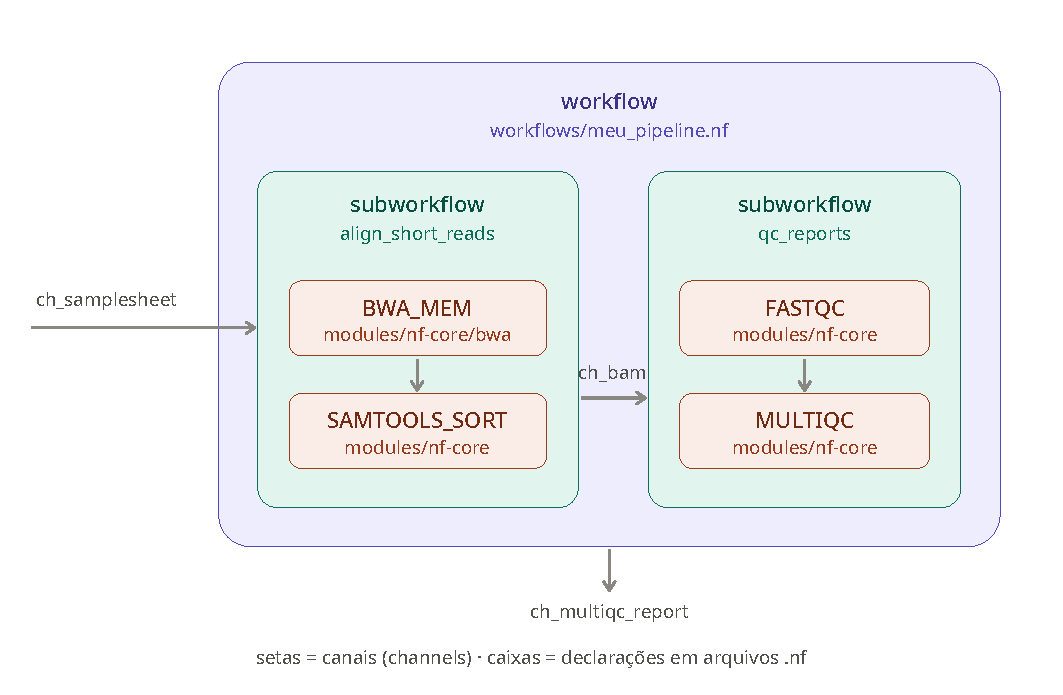
\includegraphics[keepaspectratio]{index_files/mediabag/images/nextflow_workflow_subworkflow_module_structure.pdf}}

\section{Examinando um script
nextflow}\label{examinando-um-script-nextflow}

Fornecemos um script de workflow funcional, embora minimalista, chamado
\href{../hello_nextflow/hello-world.nf}{hello-world.nf} que escreve
`Hello World!' com Nextflow.

Para começar, vamos abrir o script do fluxo de trabalho para que você
tenha uma noção de como ele está estruturado. Então vamos executá-lo e
procurar suas saídas.

\begin{tcolorbox}[enhanced jigsaw, arc=.35mm, bottomrule=.15mm, bottomtitle=1mm, breakable, colback=white, colbacktitle=quarto-callout-note-color!10!white, colframe=quarto-callout-note-color-frame, coltitle=black, left=2mm, leftrule=.75mm, opacityback=0, opacitybacktitle=0.6, rightrule=.15mm, title=\textcolor{quarto-callout-note-color}{\faInfo}\hspace{0.5em}{Ver conteúdo de \texttt{hello-world.nf}}, titlerule=0mm, toprule=.15mm, toptitle=1mm]

\begin{Shaded}
\begin{Highlighting}[]
\NormalTok{\#}\OperatorTok{!}\StringTok{/usr/}\NormalTok{bin}\OperatorTok{/}\NormalTok{env nextflow}

\CommentTok{/*}
\CommentTok{ * Use echo to print \textquotesingle{}Hello World!\textquotesingle{} to a file}
\CommentTok{ */}
\NormalTok{process sayHello }\OperatorTok{\{}

\NormalTok{    output}\OperatorTok{:}
\NormalTok{    path }\StringTok{\textquotesingle{}output.txt\textquotesingle{}}

\NormalTok{    script}\OperatorTok{:}
    \StringTok{"""}
\StringTok{    echo \textquotesingle{}Hello World!\textquotesingle{} \textgreater{} output.txt}
\StringTok{    """}
\OperatorTok{\}}

\NormalTok{workflow }\OperatorTok{\{}

\NormalTok{    main}\OperatorTok{:}
    \CommentTok{// emit a greeting}
    \FunctionTok{sayHello}\OperatorTok{()}

\OperatorTok{\}}
\end{Highlighting}
\end{Shaded}

\end{tcolorbox}

\begin{tcolorbox}[enhanced jigsaw, arc=.35mm, bottomrule=.15mm, bottomtitle=1mm, breakable, colback=white, colbacktitle=quarto-callout-tip-color!10!white, colframe=quarto-callout-tip-color-frame, coltitle=black, left=2mm, leftrule=.75mm, opacityback=0, opacitybacktitle=0.6, rightrule=.15mm, title=\textcolor{quarto-callout-tip-color}{\faLightbulb}\hspace{0.5em}{Dica}, titlerule=0mm, toprule=.15mm, toptitle=1mm]

Um script de fluxo de trabalho Nextflow normalmente inclui uma ou mais
definições de process e o workflow em si, além de alguns blocos
opcionais (não presentes aqui) que apresentaremos mais tarde.

\end{tcolorbox}

\subsection{Componentes do
hello-world.nf}\label{componentes-do-hello-world.nf}

\begin{itemize}
\tightlist
\item
  \textbf{\texttt{process}}: O primeiro bloco de código descreve um
  \texttt{process}. O corpo do processo deve conter um bloco script que
  especifica o comando a ser executado, \textbf{que pode ser qualquer
  coisa que você seria capaz de executar em um terminal de linha de
  comando.}

  \begin{itemize}
  \tightlist
  \item
    Estrutura mínima

    \begin{itemize}
    \tightlist
    \item
      Nome \texttt{sayHello}
    \item
      output neste caso inclui o qualificador \texttt{path}
    \item
      script o que será executado
    \end{itemize}
  \end{itemize}
\item
  \textbf{\texttt{workflow}}: O segundo bloco de código descreve o
  workflow em si. A definição de fluxo de trabalho começa com a
  palavra-chave workflow, seguida por um nome opcional, depois o corpo
  do fluxo de trabalho delimitado por chaves.
\end{itemize}

\subsection{Execute o workflow}\label{execute-o-workflow}

Lance o fluxo de trabalho e monitore a execução, no terminal, execute o
seguinte comando:

\begin{Shaded}
\begin{Highlighting}[]
\ExtensionTok{nextflow}\NormalTok{ run hello{-}world.nf}
\end{Highlighting}
\end{Shaded}

\subsection{Encontre a saída e os logs de
execução}\label{encontre-a-sauxedda-e-os-logs-de-execuuxe7uxe3o}

Quando você executa o Nextflow, é criado um diretório chamado
\texttt{work} onde ele escreverá todos os arquivos gerados durante a
execução.

Dentro do diretório \texttt{work}, para cada chamada de processo, o
Nextflow cria um subdiretório aninhado, nomeado com um hash para
torná-lo único, onde preparará todas as entradas necessárias, escreverá
arquivos auxiliares e escreverá logs e quaisquer saídas do processo.

Para examinar o diretório work execute:

\begin{Shaded}
\begin{Highlighting}[]
\ExtensionTok{tree} \AttributeTok{{-}a}\NormalTok{ work}
\end{Highlighting}
\end{Shaded}

\begin{itemize}
\tightlist
\item
  \textbf{.command.begin}: Metadados relacionados ao início da execução
  da chamada do processo
\item
  \textbf{.command.err}: Mensagens de erro (stderr) emitidas pela
  chamada do processo
\item
  \textbf{.command.log}: Saída de log completa emitida pela chamada do
  processo
\item
  \textbf{.command.out}: Saída regular (stdout) pela chamada do processo
\item
  \textbf{.command.run}: Script completo executado pelo Nextflow para
  executar a chamada do processo
\item
  \textbf{.command.sh}: O comando que foi realmente executado pela
  chamada do processo
\item
  \textbf{.exitcode}: O código de saída resultante do comando
\end{itemize}

O arquivo \texttt{.command.sh} é especialmente útil porque informa o
comando principal que o Nextflow executou, \emph{não incluindo toda a
contabilidade e configuração de tarefa/ambiente}.

Caso o workflow seja executado novamente um novo subdiretório com um
conjunto completo de arquivos de saída e log será criado para cada
execução. Isso mostra que executar o mesmo fluxo de trabalho várias
vezes não sobrescreverá os resultados de execuções anteriores.

\section{Aprimorando o Hello world}\label{aprimorando-o-hello-world}

\subsection{Publique outputs}\label{publique-outputs}

A saída produzida pelo nosso pipeline está enterrada no diretório
\texttt{work} várias camadas abaixo. Isso é feito propositalmente; o
Nextflow está no controle desse diretório e não devemos interagir com
ele. No entanto, isso torna inconveniente recuperar saídas que nos
interessam.

Para contornar isso, podemos publicar os outputs em um diretório
designado usando definições de saída em nível de workflow.

\subsection{Uso básico}\label{uso-buxe1sico}

Isso vai envolver dois novos pedaços de código:

\begin{enumerate}
\def\labelenumi{\arabic{enumi}.}
\tightlist
\item
  Um bloco \texttt{publish}: dentro do corpo do workflow, declarando
  saídas de processo.
\item
  Um bloco \texttt{output} no script especificando opções de saída como
  modo e localização.
\end{enumerate}

Adicione o bloco publish:

\section{Depois}

\begin{Shaded}
\begin{Highlighting}[]
\NormalTok{workflow }\OperatorTok{\{}

\NormalTok{    main}\OperatorTok{:}
    \CommentTok{// emite uma saudação}
    \FunctionTok{sayHello}\OperatorTok{()}

\NormalTok{    publish}\OperatorTok{:}
\NormalTok{    first\_output }\OperatorTok{=}\NormalTok{ sayHello}\OperatorTok{.}\NormalTok{out}
\OperatorTok{\}}
\end{Highlighting}
\end{Shaded}

\section{Antes}

\begin{Shaded}
\begin{Highlighting}[]
\NormalTok{workflow }\OperatorTok{\{}

\NormalTok{    main}\OperatorTok{:}
    \CommentTok{// emite uma saudação}
    \FunctionTok{sayHello}\OperatorTok{()}
\OperatorTok{\}}
\end{Highlighting}
\end{Shaded}

\begin{tcolorbox}[enhanced jigsaw, arc=.35mm, bottomrule=.15mm, bottomtitle=1mm, breakable, colback=white, colbacktitle=quarto-callout-note-color!10!white, colframe=quarto-callout-note-color-frame, coltitle=black, left=2mm, leftrule=.75mm, opacityback=0, opacitybacktitle=0.6, rightrule=.15mm, title=\textcolor{quarto-callout-note-color}{\faInfo}\hspace{0.5em}{Nota}, titlerule=0mm, toprule=.15mm, toptitle=1mm]

Você vê que podemos nos referir à saída do processo simplesmente fazendo
sayHello().out, e atribuir a ela um nome arbitrário, first\_output.

\end{tcolorbox}

Adicione o bloco \texttt{output} ao script onde o caminho do diretório
de saída será especificado:

\section{Depois}

\begin{Shaded}
\begin{Highlighting}[]
\NormalTok{workflow }\OperatorTok{\{}

\NormalTok{    main}\OperatorTok{:}
    \CommentTok{// emite uma saudação}
    \FunctionTok{sayHello}\OperatorTok{()}

\NormalTok{    publish}\OperatorTok{:}
\NormalTok{    first\_output }\OperatorTok{=}\NormalTok{ sayHello}\OperatorTok{.}\NormalTok{out}
\OperatorTok{\}}

\NormalTok{output }\OperatorTok{\{}
\NormalTok{    first\_output }\OperatorTok{\{}
\NormalTok{        path }\StringTok{\textquotesingle{}hello\_world\textquotesingle{}}
    \OperatorTok{\}}
\OperatorTok{\}}
\end{Highlighting}
\end{Shaded}

\section{Antes}

\begin{Shaded}
\begin{Highlighting}[]
\NormalTok{workflow }\OperatorTok{\{}

\NormalTok{    main}\OperatorTok{:}
    \CommentTok{// emite uma saudação}
    \FunctionTok{sayHello}\OperatorTok{()}

\NormalTok{    publish}\OperatorTok{:}
\NormalTok{    first\_output }\OperatorTok{=}\NormalTok{ sayHello}\OperatorTok{.}\NormalTok{out}
\OperatorTok{\}}
\end{Highlighting}
\end{Shaded}

Execute o workflow modificado:

\begin{Shaded}
\begin{Highlighting}[]
\ExtensionTok{nextflow}\NormalTok{ run hello{-}world.nf}
\end{Highlighting}
\end{Shaded}

\section{Usando inputs variáveis}\label{usando-inputs-variuxe1veis}

Em seu estado atual, nosso fluxo de trabalho usa uma saudação codificada
no comando do processo. Queremos adicionar alguma flexibilidade usando
uma variável de entrada, para que possamos mudar mais facilmente a
saudação em tempo de execução.

Isso requer que façamos três conjuntos de mudanças em nosso script:

\begin{enumerate}
\def\labelenumi{\arabic{enumi}.}
\tightlist
\item
  Alterar o processo para esperar uma entrada variável
\item
  Configurar um parâmetro de linha de comando para capturar a entrada do
  usuário
\item
  Passar a entrada para o processo no corpo do fluxo de trabalho
\end{enumerate}

Vamos fazer essas mudanças uma de cada vez.

Primeiro, vamos adaptar a definição do processo para aceitar uma entrada
chamada greeting.

\section{Depois}

\begin{Shaded}
\begin{Highlighting}[]
\NormalTok{process sayHello }\OperatorTok{\{}

\NormalTok{    input}\OperatorTok{:}
\NormalTok{    val greeting}

\NormalTok{    output}\OperatorTok{:}
\NormalTok{    path }\StringTok{\textquotesingle{}output.txt\textquotesingle{}}
\end{Highlighting}
\end{Shaded}

\section{Antes}

\begin{Shaded}
\begin{Highlighting}[]
\NormalTok{process sayHello }\OperatorTok{\{}

\NormalTok{    output}\OperatorTok{:}
\NormalTok{    path }\StringTok{\textquotesingle{}output.txt\textquotesingle{}}
\end{Highlighting}
\end{Shaded}

Agora trocamos o valor codificado original pelo valor da variável de
entrada que esperamos receber.

\section{Depois}

\begin{Shaded}
\begin{Highlighting}[]
\NormalTok{    script}\OperatorTok{:}
    \StringTok{"""}
\StringTok{    echo \textquotesingle{}}\SpecialStringTok{$\{}\NormalTok{greeting}\SpecialStringTok{\}}\StringTok{\textquotesingle{} \textgreater{} output.txt}
\StringTok{    """}
\end{Highlighting}
\end{Shaded}

\section{Antes}

\begin{Shaded}
\begin{Highlighting}[]
\NormalTok{    script}\OperatorTok{:}
    \StringTok{"""}
\StringTok{    echo \textquotesingle{}Hello World!\textquotesingle{} \textgreater{} output.txt}
\StringTok{    """}
\end{Highlighting}
\end{Shaded}

Aqui, queremos criar um parâmetro chamado \texttt{-\/-input}. Em
princípio podemos escrevê-lo em qualquer lugar, mas podemos colocá-lo
diretamente em \texttt{sayHello()}.

No bloco do fluxo de trabalho, faça a seguinte alteração de código:

\section{Depois}

\begin{Shaded}
\begin{Highlighting}[]
    \CommentTok{// emite uma saudação}
    \FunctionTok{sayHello}\OperatorTok{(}\NormalTok{params}\OperatorTok{.}\NormalTok{input}\OperatorTok{)}
\end{Highlighting}
\end{Shaded}

\section{Antes}

\begin{Shaded}
\begin{Highlighting}[]
    \CommentTok{// emite uma saudação}
    \FunctionTok{sayHello}\OperatorTok{()}
\end{Highlighting}
\end{Shaded}

Agora execute o workflow

\begin{Shaded}
\begin{Highlighting}[]
\ExtensionTok{nextflow}\NormalTok{ run hello{-}world.nf }\AttributeTok{{-}{-}input} \StringTok{\textquotesingle{}Oi mundo!\textquotesingle{}}
\end{Highlighting}
\end{Shaded}

\chapter{Gerenciando execução do
workflow}\label{gerenciando-execuuxe7uxe3o-do-workflow}

Saber como lançar fluxos de trabalho e recuperar saídas é ótimo, mas
você rapidamente descobrirá que há alguns outros aspectos do
gerenciamento de fluxo de trabalho que tornarão sua vida mais fácil,
especialmente se você estiver desenvolvendo seus próprios fluxos de
trabalho.

Aqui mostramos como usar o recurso -resume para quando você precisar
relançar o mesmo fluxo de trabalho, como inspecionar o log de execuções
passadas com nextflow log, e como excluir diretórios work mais antigos
com nextflow clean.

\subsection{\texorpdfstring{Relance um fluxo de trabalho com
\texttt{-resume}}{Relance um fluxo de trabalho com -resume}}\label{relance-um-fluxo-de-trabalho-com--resume}

Às vezes, você vai querer executar novamente um pipeline que já lançou
anteriormente sem refazer nenhuma etapa que já foi concluída com
sucesso.

O Nextflow tem uma opção chamada -resume que permite fazer isso.
Especificamente, neste modo, quaisquer processos que já foram executados
com exatamente o mesmo código, configurações e entradas serão ignorados.
Isso significa que o Nextflow só executará processos que você adicionou
ou modificou desde a última execução, ou aos quais você está fornecendo
novas configurações ou entradas.

Para usá-lo, basta adicionar -resume ao seu comando e executá-lo:

\begin{Shaded}
\begin{Highlighting}[]
\ExtensionTok{nextflow}\NormalTok{ run hello{-}world.nf }\AttributeTok{{-}{-}input} \StringTok{\textquotesingle{}Konnichiwa!\textquotesingle{}} \AttributeTok{{-}resume}
\end{Highlighting}
\end{Shaded}

\subsection{Inspecione o log ou limpe execuções
passadas}\label{inspecione-o-log-ou-limpe-execuuxe7uxf5es-passadas}

Sempre que você lança um fluxo de trabalho nextflow, uma linha é escrita
em um arquivo de log chamado history, em um diretório oculto chamado
.nextflow no diretório de trabalho atual.

\begin{tcolorbox}[enhanced jigsaw, arc=.35mm, bottomrule=.15mm, bottomtitle=1mm, breakable, colback=white, colbacktitle=quarto-callout-note-color!10!white, colframe=quarto-callout-note-color-frame, coltitle=black, left=2mm, leftrule=.75mm, opacityback=0, opacitybacktitle=0.6, rightrule=.15mm, title=\textcolor{quarto-callout-note-color}{\faInfo}\hspace{0.5em}{Ver exemplo do arquivo \texttt{.nextflow/history}}, titlerule=0mm, toprule=.15mm, toptitle=1mm]

\begin{Shaded}
\begin{Highlighting}[]
\NormalTok{2024{-}11{-}05 10:32:15 5m 23s  golden\_cantor   OK  a1b2c3d4    1a2b3c4d{-}...    nextflow run hello{-}world.nf}
\NormalTok{2024{-}11{-}05 10:41:07 3m 12s  elegant\_curie   OK  a1b2c3d4    5e6f7a8b{-}...    nextflow run hello{-}world.nf {-}{-}input \textquotesingle{}Bonjour!\textquotesingle{}}
\NormalTok{2024{-}11{-}05 11:02:44 4m 58s  naughty\_lorenz  ERR a1b2c3d4    9c0d1e2f{-}...    nextflow run hello{-}world.nf {-}{-}input \textquotesingle{}Konnichiwa!\textquotesingle{} {-}resume}
\end{Highlighting}
\end{Shaded}

Cada linha: timestamp, duração, nome da execução, status, ID de revisão,
ID de sessão, linha de comando.

\end{tcolorbox}

Este arquivo fornece o timestamp, nome da execução, status, ID de
revisão, ID de sessão e linha de comando completa para cada execução do
Nextflow que foi lançada a partir do diretório de trabalho atual.

Uma maneira mais conveniente de acessar essas informações é usar o
comando nextflow log.

\begin{Shaded}
\begin{Highlighting}[]
\ExtensionTok{nextflow}\NormalTok{ log}
\end{Highlighting}
\end{Shaded}

Durante o processo de desenvolvimento, você normalmente executará seu
rascunho de pipeline um grande número de vezes, o que pode levar a um
acúmulo de muitos arquivos em muitos subdiretórios.

Felizmente, o Nextflow inclui um subcomando útil clean que pode excluir
automaticamente os subdiretórios work de execuções passadas que você não
se importa mais.

Existem várias opções para determinar o que excluir.

Aqui mostramos um exemplo que exclui todos os subdiretórios de execuções
antes de uma determinada execução, especificada usando seu nome de
execução.

Primeiro usamos a flag de execução de teste -n para verificar o que será
excluído dado o comando:

\begin{Shaded}
\begin{Highlighting}[]
\ExtensionTok{nextflow}\NormalTok{ clean }\AttributeTok{{-}before}\NormalTok{ golden\_cantor }\AttributeTok{{-}n}
\end{Highlighting}
\end{Shaded}

Se a saída parecer como esperado e você quiser prosseguir com a
exclusão, execute novamente o comando com a flag -f em vez de -n:

\begin{Shaded}
\begin{Highlighting}[]
\ExtensionTok{nextflow}\NormalTok{ clean }\AttributeTok{{-}before}\NormalTok{ golden\_cantor }\AttributeTok{{-}f}
\end{Highlighting}
\end{Shaded}

\chapter{Componentes de um Workflow}\label{componentes-de-um-workflow}

\section{Channels}\label{channels}

Na maioria dos pipelines realistas, queremos processar múltiplos valores
(vários arquivos FASTQ, por exemplo), então precisamos de uma maneira
mais sofisticada de lidar com entradas.

É para isso que servem os canais do Nextflow. Canais são filas
projetadas para lidar com entradas eficientemente e transportá-las de
uma etapa para outra em fluxos de trabalho de múltiplas etapas, ao mesmo
tempo que fornecem paralelismo integrado e muitos benefícios adicionais.

\subsection{Forneça entradas variáveis através de um canal
explicitamente}\label{forneuxe7a-entradas-variuxe1veis-atravuxe9s-de-um-canal-explicitamente}

Existem várias fábricas de canais que podemos usar para configurar um
canal. Para manter as coisas simples por enquanto, vamos usar a fábrica
de canais mais básica, chamada channel.of, que criará um canal contendo
um único valor. Funcionalmente, isso será semelhante a como tínhamos
configurado antes, mas em vez de ter o Nextflow criando um canal
implicitamente, estamos fazendo isso explicitamente agora.

Adicione o channel greeting\_ch em
\href{../hello_nextflow/hello-channels.nf}{hello\_channels.nf}:

\begin{Shaded}
\begin{Highlighting}[]

\NormalTok{workflow }\OperatorTok{\{}

\NormalTok{    main}\OperatorTok{:}
    \CommentTok{// cria um canal para entradas}
\NormalTok{    greeting\_ch }\OperatorTok{=}\NormalTok{ channel}\OperatorTok{.}\FunctionTok{of}\OperatorTok{(}\StringTok{\textquotesingle{}Hello\textquotesingle{}}\OperatorTok{,}\StringTok{\textquotesingle{}Bonjour\textquotesingle{}}\OperatorTok{,}\StringTok{\textquotesingle{}Hola\textquotesingle{}}\OperatorTok{,} \StringTok{"Oi"}\OperatorTok{)}
    \CommentTok{// emite uma saudação}
    \FunctionTok{sayHello}\OperatorTok{(}\NormalTok{greeting\_ch}\OperatorTok{)}

\NormalTok{    publish}\OperatorTok{:}
\NormalTok{    first\_output }\OperatorTok{=}\NormalTok{ sayHello}\OperatorTok{.}\NormalTok{out}
\OperatorTok{\}}
\end{Highlighting}
\end{Shaded}

Isso cria um canal chamado greeting\_ch usando a fábrica de canais
channel.of(), que configura um canal de fila simples, e carrega a string
`Hello Channels!' para usar como o valor da saudação.

Execute o workflow:

\begin{Shaded}
\begin{Highlighting}[]
\ExtensionTok{nextflow}\NormalTok{ run hello{-}channels.nf}
\end{Highlighting}
\end{Shaded}

Os canais do Nextflow são construídos de uma maneira que nos permite
operar em seu conteúdo usando operadores, que cobriremos em detalhes
mais tarde neste capítulo.

Por enquanto, vamos apenas mostrar como usar um operador super simples
chamado \texttt{view()} para inspecionar o conteúdo de um canal. Você
pode pensar em \texttt{view()} como uma ferramenta de depuração, como
uma instrução \texttt{print()} em Python, ou seu equivalente em outras
linguagens.

Adicione esta pequena linha ao bloco workflow:

\begin{Shaded}
\begin{Highlighting}[]
\NormalTok{workflow }\OperatorTok{\{}

\NormalTok{    main}\OperatorTok{:}
    \CommentTok{// cria um canal para entradas}
\NormalTok{    greeting\_ch }\OperatorTok{=}\NormalTok{ channel}\OperatorTok{.}\FunctionTok{of}\OperatorTok{(}\StringTok{\textquotesingle{}Hello Channels!\textquotesingle{}}\OperatorTok{)}
                         \OperatorTok{.}\FunctionTok{view}\OperatorTok{()}
    \CommentTok{// emite uma saudação}
    \FunctionTok{sayHello}\OperatorTok{(}\NormalTok{greeting\_ch}\OperatorTok{)}

\NormalTok{    publish}\OperatorTok{:}
\NormalTok{    first\_output }\OperatorTok{=}\NormalTok{ sayHello}\OperatorTok{.}\NormalTok{out}
\OperatorTok{\}}
\end{Highlighting}
\end{Shaded}

Agora execute o fluxo de trabalho novamente:

\begin{Shaded}
\begin{Highlighting}[]
\NormalTok{nextflow run hello}\OperatorTok{{-}}\NormalTok{channels}\OperatorTok{.}\NormalTok{nf}
\end{Highlighting}
\end{Shaded}

Como você pode ver, isso exibe o conteúdo do canal no console. Aqui
temos apenas um elemento, mas quando começarmos a carregar múltiplos
valores no canal na próxima seção, você verá que isso está configurado
para exibir um elemento por linha.

\pandocbounded{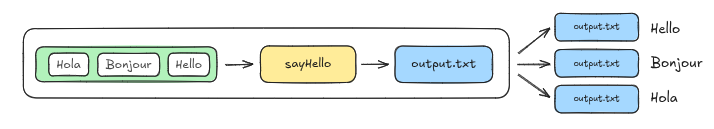
\includegraphics[keepaspectratio]{images/channels_hellonf.png}}

\section{Workflows}\label{workflows}

A maioria dos fluxos de trabalho do mundo real envolve mais de uma
etapa. Neste módulo de treinamento, você aprenderá como conectar
processos em um fluxo de trabalho com múltiplas etapas.

Agora veremos como realizar o seguinte:

\begin{enumerate}
\def\labelenumi{\arabic{enumi}.}
\tightlist
\item
  Fazer os dados fluírem de um processo para o próximo
\item
  Coletar saídas de múltiplas chamadas de processo em uma única chamada
  de processo
\item
  Passar parâmetros adicionais para um processo
\item
  Lidar com múltiplas saídas provenientes de um processo
\end{enumerate}

Para demonstrar, continuaremos construindo sobre o exemplo Hello World
agnóstico de domínio das Partes 1 e 2. Desta vez, faremos as seguintes
alterações em nosso fluxo de trabalho para refletir melhor como as
pessoas constroem fluxos de trabalho reais:

\begin{enumerate}
\def\labelenumi{\arabic{enumi}.}
\tightlist
\item
  Adicionar uma segunda etapa que converte a saudação para maiúsculas.
\item
  Adicionar uma terceira etapa que coleta todas as saudações
  transformadas e as escreve em um único arquivo.
\item
  Adicionar um parâmetro para nomear o arquivo de saída final e passá-lo
  como uma entrada secundária para a etapa de coleta.
\item
  Fazer a etapa de coleta também reportar uma estatística simples sobre
  o que foi processado.
\end{enumerate}

Execute \href{../hello_nextflow/hello-workflow.nf}{hello-workflow.nf} :

\begin{Shaded}
\begin{Highlighting}[]
\ExtensionTok{nextflow}\NormalTok{ run hello{-}workflow.nf}
\end{Highlighting}
\end{Shaded}

Este diagrama resume a operação atual do fluxo de trabalho. Deve parecer
familiar, exceto que agora estamos mostrando explicitamente que as
saídas do processo são empacotadas em um canal, assim como as entradas
foram. Vamos colocar esse canal de saída em bom uso em um minuto.

\pandocbounded{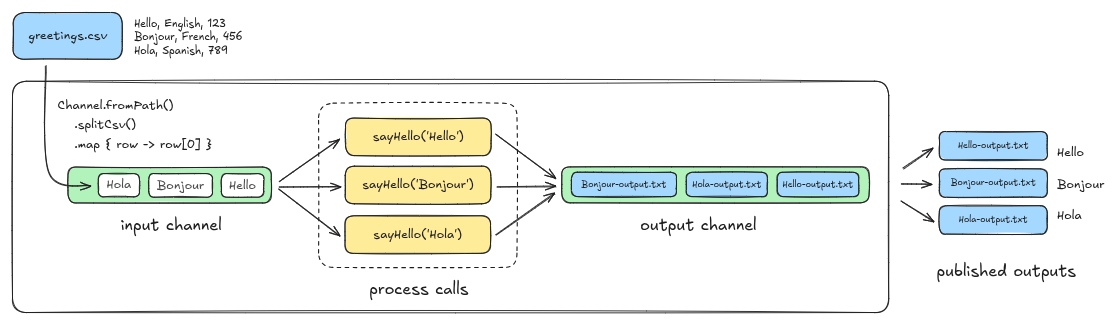
\includegraphics[keepaspectratio]{images/workflow_hellonf.png}}

\section{Adicionando uma segunda
etapa}\label{adicionando-uma-segunda-etapa}

Vamos adicionar uma etapa para converter cada saudação para maiúsculas.

\pandocbounded{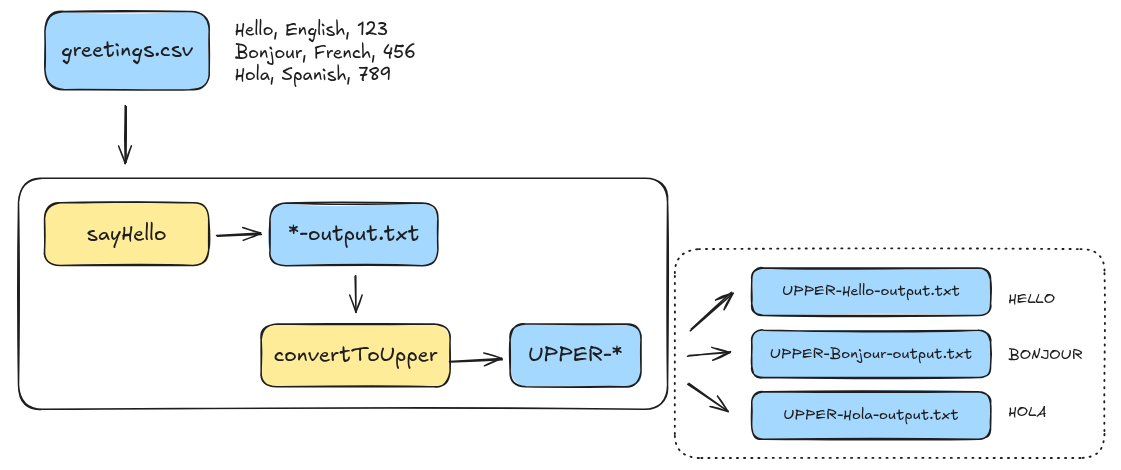
\includegraphics[keepaspectratio]{images/workflow_translate_hellonf.png}}

Para isso, precisamos fazer três coisas:

\begin{itemize}
\tightlist
\item
  Definir o comando que vamos usar para fazer a conversão para
  maiúsculas.
\item
  Escrever um novo processo que envolve o comando de conversão para
  maiúsculas.
\item
  Chamar o novo processo no bloco workflow e configurá-lo para receber a
  saída do processo sayHello() como entrada.
\end{itemize}

\begin{enumerate}
\def\labelenumi{\arabic{enumi}.}
\tightlist
\item
  Comando de conversão para maiúsculas e teste-o no terminal:
\end{enumerate}

\begin{Shaded}
\begin{Highlighting}[]
\FunctionTok{tr} \StringTok{\textquotesingle{}[a{-}z]\textquotesingle{}} \StringTok{\textquotesingle{}[A{-}Z]\textquotesingle{}}
\end{Highlighting}
\end{Shaded}

\begin{enumerate}
\def\labelenumi{\arabic{enumi}.}
\setcounter{enumi}{1}
\tightlist
\item
  Adicionando um novo processo em nosso workflow que irá executar esse
  comando
\end{enumerate}

\begin{Shaded}
\begin{Highlighting}[]
\CommentTok{/*}
\CommentTok{ * Use uma ferramenta de substituição de texto para converter a saudação para maiúsculas}
\CommentTok{ */}
\NormalTok{process convertToUpper }\OperatorTok{\{}

\NormalTok{    input}\OperatorTok{:}
\NormalTok{    path input\_file}

\NormalTok{    output}\OperatorTok{:}
\NormalTok{    path }\StringTok{"UPPER{-}}\SpecialStringTok{$\{}\NormalTok{input\_file}\SpecialStringTok{\}}\StringTok{"}

\NormalTok{    script}\OperatorTok{:}
    \StringTok{"""}
\StringTok{    cat \textquotesingle{}}\SpecialStringTok{$\{}\NormalTok{input\_file}\SpecialStringTok{\}}\StringTok{\textquotesingle{} | tr \textquotesingle{}[a{-}z]\textquotesingle{} \textquotesingle{}[A{-}Z]\textquotesingle{} \textgreater{} \textquotesingle{}UPPER{-}}\SpecialStringTok{$\{}\NormalTok{input\_file}\SpecialStringTok{\}}\StringTok{\textquotesingle{}}
\StringTok{    """}
\OperatorTok{\}}
\end{Highlighting}
\end{Shaded}

\begin{tcolorbox}[enhanced jigsaw, arc=.35mm, bottomrule=.15mm, bottomtitle=1mm, breakable, colback=white, colbacktitle=quarto-callout-tip-color!10!white, colframe=quarto-callout-tip-color-frame, coltitle=black, left=2mm, leftrule=.75mm, opacityback=0, opacitybacktitle=0.6, rightrule=.15mm, title=\textcolor{quarto-callout-tip-color}{\faLightbulb}\hspace{0.5em}{Dica}, titlerule=0mm, toprule=.15mm, toptitle=1mm]

Neste, componhamos o segundo nome de arquivo de saída com base no nome
do arquivo de entrada, de forma similar ao que fizemos originalmente
para a saída do primeiro processo.

\end{tcolorbox}

\begin{enumerate}
\def\labelenumi{\arabic{enumi}.}
\setcounter{enumi}{2}
\tightlist
\item
  Adicione uma chamada ao novo processo no bloco workflow
\end{enumerate}

\begin{Shaded}
\begin{Highlighting}[]
\NormalTok{workflow }\OperatorTok{\{}

\NormalTok{    main}\OperatorTok{:}
    \CommentTok{// cria um canal para entradas a partir de um arquivo CSV}
\NormalTok{    greeting\_ch }\OperatorTok{=}\NormalTok{ channel}\OperatorTok{.}\FunctionTok{fromPath}\OperatorTok{(}\NormalTok{params}\OperatorTok{.}\NormalTok{input}\OperatorTok{)}
                        \OperatorTok{.}\FunctionTok{splitCsv}\OperatorTok{()}
                        \OperatorTok{.}\FunctionTok{map} \OperatorTok{\{}\NormalTok{ line }\OperatorTok{{-}\textgreater{}}\NormalTok{ line}\OperatorTok{[}\DecValTok{0}\OperatorTok{]} \OperatorTok{\}}
    \CommentTok{// emite uma saudação}
    \FunctionTok{sayHello}\OperatorTok{(}\NormalTok{greeting\_ch}\OperatorTok{)}
    \CommentTok{// converte a saudação para maiúsculas}
    \FunctionTok{convertToUpper}\OperatorTok{()}

\NormalTok{    publish}\OperatorTok{:}
\NormalTok{    first\_output }\OperatorTok{=}\NormalTok{ sayHello}\OperatorTok{.}\NormalTok{out}
\OperatorTok{\}}
\end{Highlighting}
\end{Shaded}

\begin{enumerate}
\def\labelenumi{\arabic{enumi}.}
\setcounter{enumi}{3}
\tightlist
\item
  Passe a saída do primeiro processo para o segundo processo
\end{enumerate}

\begin{Shaded}
\begin{Highlighting}[]
    \CommentTok{// converte a saudação para maiúsculas}
    \FunctionTok{convertToUpper}\OperatorTok{(}\NormalTok{sayHello}\OperatorTok{.}\NormalTok{out}\OperatorTok{)}
\end{Highlighting}
\end{Shaded}

\begin{enumerate}
\def\labelenumi{\arabic{enumi}.}
\setcounter{enumi}{4}
\tightlist
\item
  Configure a publicação de saída do fluxo de trabalho
\end{enumerate}

\begin{Shaded}
\begin{Highlighting}[]

\NormalTok{    publish}\OperatorTok{:}
\NormalTok{    first\_output }\OperatorTok{=}\NormalTok{ sayHello}\OperatorTok{.}\NormalTok{out}
\NormalTok{    uppercased }\OperatorTok{=}\NormalTok{ convertToUpper}\OperatorTok{.}\NormalTok{out}
\OperatorTok{\}}
\end{Highlighting}
\end{Shaded}

\begin{Shaded}
\begin{Highlighting}[]
\NormalTok{output }\OperatorTok{\{}
\NormalTok{    first\_output }\OperatorTok{\{}
\NormalTok{        path }\StringTok{\textquotesingle{}hello\_workflow\textquotesingle{}}
\NormalTok{        mode }\StringTok{\textquotesingle{}copy\textquotesingle{}}
    \OperatorTok{\}}
\NormalTok{    uppercased }\OperatorTok{\{}
\NormalTok{        path }\StringTok{\textquotesingle{}hello\_workflow\textquotesingle{}}
\NormalTok{        mode }\StringTok{\textquotesingle{}copy\textquotesingle{}}
    \OperatorTok{\}}
\OperatorTok{\}}
\end{Highlighting}
\end{Shaded}

Execute o fluxo de trabalho com -resume

\begin{Shaded}
\begin{Highlighting}[]
\ExtensionTok{nextflow}\NormalTok{ run hello{-}workflow.nf }\AttributeTok{{-}resume}
\end{Highlighting}
\end{Shaded}

\section{Módulos}\label{muxf3dulos}

É uma boa prática armazenar seus módulos em um diretório específico.
Você pode chamar esse diretório de qualquer nome, mas a convenção é
chamá-lo de modules/.

\begin{Shaded}
\begin{Highlighting}[]
\FunctionTok{mkdir}\NormalTok{ modules}
\end{Highlighting}
\end{Shaded}

Na sua forma mais simples, transformar um processo existente em um
módulo é pouco mais do que uma operação de copiar e colar. Vamos criar
um esboço de arquivo para o módulo, copiar o código relevante e então
excluí-lo do arquivo principal do fluxo de trabalho.

Então tudo o que precisaremos fazer é adicionar uma declaração include
para que o Nextflow saiba trazer o código relevante em tempo de
execução.

Crie um novo arquivo chamado sayHello.nf dentro da pasta modules e cole
o processo sayHello

\texttt{modules/sayHello.nf}

\begin{Shaded}
\begin{Highlighting}[]
\CommentTok{/*}
\CommentTok{ * Usa echo para imprimir \textquotesingle{}Hello World!\textquotesingle{} em um arquivo}
\CommentTok{ */}
\NormalTok{process sayHello }\OperatorTok{\{}

\NormalTok{    input}\OperatorTok{:}
\NormalTok{    val greeting}

\NormalTok{    output}\OperatorTok{:}
\NormalTok{    path }\StringTok{"}\SpecialStringTok{$\{}\NormalTok{greeting}\SpecialStringTok{\}}\StringTok{{-}output.txt"}

\NormalTok{    script}\OperatorTok{:}
    \StringTok{"""}
\StringTok{    echo \textquotesingle{}}\SpecialStringTok{$\{}\NormalTok{greeting}\SpecialStringTok{\}}\StringTok{\textquotesingle{} \textgreater{} \textquotesingle{}}\SpecialStringTok{$\{}\NormalTok{greeting}\SpecialStringTok{\}}\StringTok{{-}output.txt\textquotesingle{}}
\StringTok{    """}
\OperatorTok{\}}
\end{Highlighting}
\end{Shaded}

Uma vez feito isso, apague o processo sayHello do arquivo de fluxo de
trabalho.

A sintaxe para incluir um processo de um módulo é bastante direta:

\begin{Shaded}
\begin{Highlighting}[]
\NormalTok{include }\OperatorTok{\{} \OperatorTok{\textless{}}\NormalTok{PROCESS\_NAME}\OperatorTok{\textgreater{}} \OperatorTok{\}}\NormalTok{ from }\StringTok{\textquotesingle{}\textless{}path\_to\_module\textgreater{}\textquotesingle{}}
\end{Highlighting}
\end{Shaded}

Vamos inserir isso acima do bloco params e preenchê-lo adequadamente.

\begin{Shaded}
\begin{Highlighting}[]
\CommentTok{// Inclui módulos}
\NormalTok{include }\OperatorTok{\{}\NormalTok{ sayHello }\OperatorTok{\}}\NormalTok{ from }\StringTok{\textquotesingle{}./modules/sayHello.nf\textquotesingle{}}

\CommentTok{/*}
\CommentTok{* Pipeline parameters}
\CommentTok{*/}
\NormalTok{params }\OperatorTok{\{}
\NormalTok{    input}\OperatorTok{:}\NormalTok{ Path }\OperatorTok{=} \StringTok{\textquotesingle{}data/greetings.csv\textquotesingle{}}
\NormalTok{    batch}\OperatorTok{:} \BuiltInTok{String} \OperatorTok{=} \StringTok{\textquotesingle{}batch\textquotesingle{}}
\OperatorTok{\}}
\end{Highlighting}
\end{Shaded}

Execute o fluxo de trabalho

\begin{Shaded}
\begin{Highlighting}[]
\NormalTok{nextflow run hello}\OperatorTok{{-}}\NormalTok{modules}\OperatorTok{.}\NormalTok{nf }\OperatorTok{{-}}\NormalTok{resume }
\end{Highlighting}
\end{Shaded}

\begin{tcolorbox}[enhanced jigsaw, arc=.35mm, bottomrule=.15mm, bottomtitle=1mm, breakable, colback=white, colbacktitle=quarto-callout-note-color!10!white, colframe=quarto-callout-note-color-frame, coltitle=black, left=2mm, leftrule=.75mm, opacityback=0, opacitybacktitle=0.6, rightrule=.15mm, title=\textcolor{quarto-callout-note-color}{\faInfo}\hspace{0.5em}{Nota}, titlerule=0mm, toprule=.15mm, toptitle=1mm]

Tentem modularizar o processo convertToUpper()

\end{tcolorbox}

\section{Containers}\label{containers}

Nas Partes 1-4 deste curso de treinamento, você aprendeu a usar os
blocos de construção básicos do Nextflow para montar um fluxo de
trabalho simples capaz de processar texto, paralelizar a execução se
houvesse múltiplas entradas e coletar os resultados para processamento
adicional.

No entanto, você estava limitado às ferramentas básicas do UNIX
disponíveis no seu ambiente. Tarefas do mundo real frequentemente
requerem várias ferramentas e pacotes não incluídos por padrão.
Normalmente, você precisaria instalar essas ferramentas, gerenciar suas
dependências e resolver quaisquer conflitos.

Tudo isso é muito tedioso e irritante, então vamos mostrar como usar
contêineres para resolver esse problema de forma muito mais conveniente.

Um contêiner é uma unidade de software leve, autônoma e executável
criada a partir de uma imagem de contêiner que inclui tudo o que é
necessário para executar uma aplicação, incluindo código, bibliotecas do
sistema e configurações. Como você pode imaginar, isso será muito útil
para tornar seus pipelines mais reproduzíveis.

Execute hello-containers.nf

\begin{Shaded}
\begin{Highlighting}[]
\ExtensionTok{nextflow}\NormalTok{ run hello{-}containers.nf}
\end{Highlighting}
\end{Shaded}

Vamos usar um ``container'' manualmente

Baixe a imagem do container

\begin{Shaded}
\begin{Highlighting}[]
\ExtensionTok{docker}\NormalTok{ pull }\StringTok{\textquotesingle{}community.wave.seqera.io/library/cowpy:1.1.5{-}{-}3db457ae1977a273\textquotesingle{}}
\end{Highlighting}
\end{Shaded}

Use o contêiner para executar cowpy como um comando único

\begin{Shaded}
\begin{Highlighting}[]
\ExtensionTok{docker}\NormalTok{ run }\AttributeTok{{-}{-}rm} \AttributeTok{{-}it} \StringTok{\textquotesingle{}community.wave.seqera.io/library/cowpy:1.1.5{-}{-}3db457ae1977a273\textquotesingle{}}\NormalTok{ /bin/bash}
\end{Highlighting}
\end{Shaded}

Execute o(s) comando(s) da ferramenta desejada
\texttt{yirdtk\ echo\ "Hello\ Containers"\ \textbar{}\ cowpy\ -c\ tux}

\subsection{Use contêineres no
Nextflow}\label{use-contuxeaineres-no-nextflow}

O Nextflow tem suporte integrado para executar processos dentro de
contêineres para permitir que você execute ferramentas que não tem
instaladas no seu ambiente de computação. Isso significa que você pode
usar qualquer imagem de contêiner que desejar para executar seus
processos, e o Nextflow cuidará de puxar a imagem, montar os dados e
executar o processo dentro dela.

Para demonstrar isso, vamos adicionar uma etapa cowpy ao pipeline que
estivemos desenvolvendo, após a etapa collectGreetings.

\pandocbounded{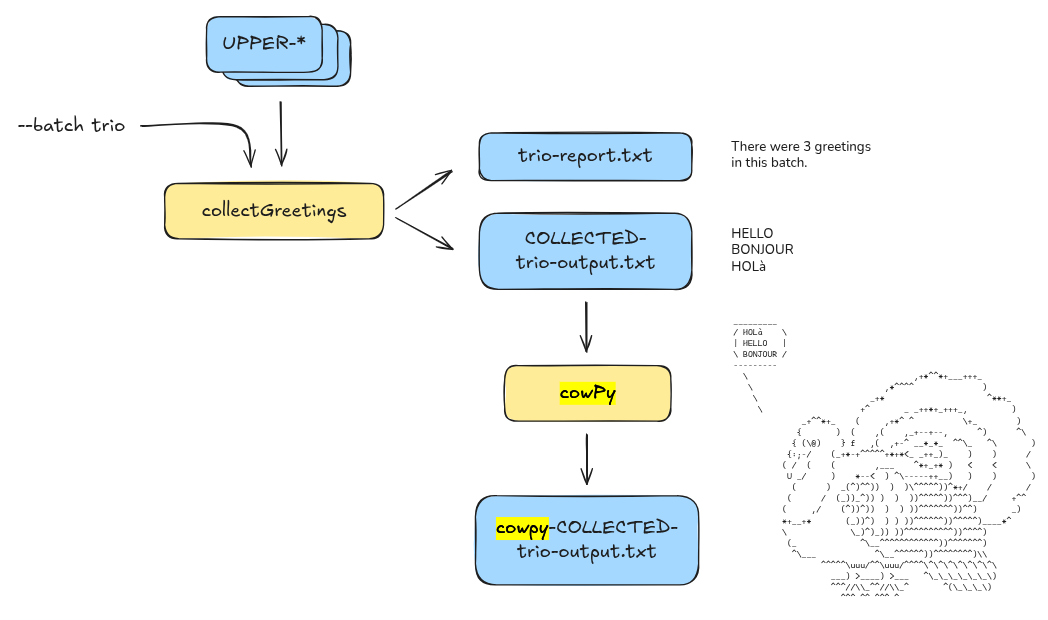
\includegraphics[keepaspectratio]{images/cowpy_hellonf.png}}

\begin{tcolorbox}[enhanced jigsaw, arc=.35mm, bottomrule=.15mm, bottomtitle=1mm, breakable, colback=white, colbacktitle=quarto-callout-note-color!10!white, colframe=quarto-callout-note-color-frame, coltitle=black, left=2mm, leftrule=.75mm, opacityback=0, opacitybacktitle=0.6, rightrule=.15mm, title=\textcolor{quarto-callout-note-color}{\faInfo}\hspace{0.5em}{Nota}, titlerule=0mm, toprule=.15mm, toptitle=1mm]

Tentem escrever o módulo cowpy.nf

\end{tcolorbox}

\begin{tcolorbox}[enhanced jigsaw, arc=.35mm, bottomrule=.15mm, bottomtitle=1mm, breakable, colback=white, colbacktitle=quarto-callout-tip-color!10!white, colframe=quarto-callout-tip-color-frame, coltitle=black, left=2mm, leftrule=.75mm, opacityback=0, opacitybacktitle=0.6, rightrule=.15mm, title=\textcolor{quarto-callout-tip-color}{\faLightbulb}\hspace{0.5em}{Mostrar resposta}, titlerule=0mm, toprule=.15mm, toptitle=1mm]

Podemos modelar nosso processo cowpy nos outros processos que escrevemos
anteriormente.

\begin{Shaded}
\begin{Highlighting}[]
\NormalTok{\#}\OperatorTok{!}\StringTok{/usr/}\NormalTok{bin}\OperatorTok{/}\NormalTok{env nextflow}

\CommentTok{// Gera arte ASCII com cowpy}
\NormalTok{process cowpy }\OperatorTok{\{}

\NormalTok{    input}\OperatorTok{:}
\NormalTok{    path input\_file}
\NormalTok{    val character}

\NormalTok{    output}\OperatorTok{:}
\NormalTok{    path }\StringTok{"cowpy{-}}\SpecialStringTok{$\{}\NormalTok{input\_file}\SpecialStringTok{\}}\StringTok{"}

\NormalTok{    script}\OperatorTok{:}
    \StringTok{"""}
\StringTok{    cat }\SpecialStringTok{$\{}\NormalTok{input\_file}\SpecialStringTok{\}}\StringTok{ | cowpy {-}c "}\SpecialStringTok{$\{}\NormalTok{character}\SpecialStringTok{\}}\StringTok{" \textgreater{} cowpy{-}}\SpecialStringTok{$\{}\NormalTok{input\_file}\SpecialStringTok{\}}
\StringTok{    """}
\end{Highlighting}
\end{Shaded}

O processo espera um input\_file contendo as saudações, bem como um
valor character.

A saída será um novo arquivo de texto contendo a arte ASCII gerada pela
ferramenta cowpy.

Adicione cowpy ao fluxo de trabalho

\begin{Shaded}
\begin{Highlighting}[]
\CommentTok{// Inclui módulos}
\NormalTok{include }\OperatorTok{\{}\NormalTok{ sayHello }\OperatorTok{\}}\NormalTok{ from }\StringTok{\textquotesingle{}./modules/sayHello.nf\textquotesingle{}}
\NormalTok{include }\OperatorTok{\{}\NormalTok{ convertToUpper }\OperatorTok{\}}\NormalTok{ from }\StringTok{\textquotesingle{}./modules/convertToUpper.nf\textquotesingle{}}
\NormalTok{include }\OperatorTok{\{}\NormalTok{ collectGreetings }\OperatorTok{\}}\NormalTok{ from }\StringTok{\textquotesingle{}./modules/collectGreetings.nf\textquotesingle{}}
\NormalTok{include }\OperatorTok{\{}\NormalTok{ cowpy }\OperatorTok{\}}\NormalTok{ from }\StringTok{\textquotesingle{}./modules/cowpy.nf\textquotesingle{}}
\end{Highlighting}
\end{Shaded}

Vamos conectar o processo cowpy() à saída do processo
collectGreetings(), que como você deve se lembrar produz duas saídas:

\begin{itemize}
\tightlist
\item
  collectGreetings.out.outfile contém o arquivo de saída
  \emph{\textless--o que queremos}
\item
  collectGreetings.out.report contém o arquivo de relatório com a
  contagem de saudações por lote
\end{itemize}

\begin{Shaded}
\begin{Highlighting}[]
\NormalTok{    main}\OperatorTok{:}
    \CommentTok{// cria um canal para entradas de um arquivo CSV}
\NormalTok{    greeting\_ch }\OperatorTok{=}\NormalTok{ channel}\OperatorTok{.}\FunctionTok{fromPath}\OperatorTok{(}\NormalTok{params}\OperatorTok{.}\NormalTok{input}\OperatorTok{)}
                        \OperatorTok{.}\FunctionTok{splitCsv}\OperatorTok{()}
                        \OperatorTok{.}\FunctionTok{map} \OperatorTok{\{}\NormalTok{ line }\OperatorTok{{-}\textgreater{}}\NormalTok{ line}\OperatorTok{[}\DecValTok{0}\OperatorTok{]} \OperatorTok{\}}
    \CommentTok{// emite uma saudação}
    \FunctionTok{sayHello}\OperatorTok{(}\NormalTok{greeting\_ch}\OperatorTok{)}
    \CommentTok{// converte a saudação para maiúsculas}
    \FunctionTok{convertToUpper}\OperatorTok{(}\NormalTok{sayHello}\OperatorTok{.}\NormalTok{out}\OperatorTok{)}
    \CommentTok{// coleta todas as saudações em um arquivo}
    \FunctionTok{collectGreetings}\OperatorTok{(}\NormalTok{convertToUpper}\OperatorTok{.}\NormalTok{out}\OperatorTok{.}\FunctionTok{collect}\OperatorTok{(),}\NormalTok{ params}\OperatorTok{.}\NormalTok{batch}\OperatorTok{)}
    \CommentTok{// gera arte ASCII das saudações com cowpy}
    \FunctionTok{cowpy}\OperatorTok{(}\NormalTok{collectGreetings}\OperatorTok{.}\NormalTok{out}\OperatorTok{.}\NormalTok{outfile}\OperatorTok{,}\NormalTok{ params}\OperatorTok{.}\NormalTok{character}\OperatorTok{)}
\end{Highlighting}
\end{Shaded}

Adicione o parâmetro character ao bloco param

\begin{Shaded}
\begin{Highlighting}[]
\CommentTok{/*}
\CommentTok{* Parâmetros do pipeline}
\CommentTok{*/}
\NormalTok{params }\OperatorTok{\{}
\NormalTok{    input}\OperatorTok{:}\NormalTok{ Path }\OperatorTok{=} \StringTok{\textquotesingle{}data/greetings.csv\textquotesingle{}}
\NormalTok{    batch}\OperatorTok{:} \BuiltInTok{String} \OperatorTok{=} \StringTok{\textquotesingle{}batch\textquotesingle{}}
\NormalTok{    character}\OperatorTok{:} \BuiltInTok{String} \OperatorTok{=} \StringTok{\textquotesingle{}turkey\textquotesingle{}}
\OperatorTok{\}}
\end{Highlighting}
\end{Shaded}

Atualize as saídas do workflow

\begin{Shaded}
\begin{Highlighting}[]

\NormalTok{    publish}\OperatorTok{:}
\NormalTok{    first\_output }\OperatorTok{=}\NormalTok{ sayHello}\OperatorTok{.}\NormalTok{out}
\NormalTok{    uppercased }\OperatorTok{=}\NormalTok{ convertToUpper}\OperatorTok{.}\NormalTok{out}
\NormalTok{    collected }\OperatorTok{=}\NormalTok{ collectGreetings}\OperatorTok{.}\NormalTok{out}\OperatorTok{.}\NormalTok{outfile}
\NormalTok{    batch\_report }\OperatorTok{=}\NormalTok{ collectGreetings}\OperatorTok{.}\NormalTok{out}\OperatorTok{.}\NormalTok{report}
\NormalTok{    cowpy\_art }\OperatorTok{=}\NormalTok{ cowpy}\OperatorTok{.}\NormalTok{out}
\end{Highlighting}
\end{Shaded}

Atualize o bloco output

\begin{Shaded}
\begin{Highlighting}[]
\NormalTok{output }\OperatorTok{\{}
\NormalTok{    first\_output }\OperatorTok{\{}
\NormalTok{        path }\StringTok{\textquotesingle{}hello\_containers/intermediates\textquotesingle{}}
\NormalTok{        mode }\StringTok{\textquotesingle{}copy\textquotesingle{}}
    \OperatorTok{\}}
\NormalTok{    uppercased }\OperatorTok{\{}
\NormalTok{        path }\StringTok{\textquotesingle{}hello\_containers/intermediates\textquotesingle{}}
\NormalTok{        mode }\StringTok{\textquotesingle{}copy\textquotesingle{}}
    \OperatorTok{\}}
\NormalTok{    collected }\OperatorTok{\{}
\NormalTok{        path }\StringTok{\textquotesingle{}hello\_containers/intermediates\textquotesingle{}}
\NormalTok{        mode }\StringTok{\textquotesingle{}copy\textquotesingle{}}
    \OperatorTok{\}}
\NormalTok{    batch\_report }\OperatorTok{\{}
\NormalTok{        path }\StringTok{\textquotesingle{}hello\_containers\textquotesingle{}}
\NormalTok{        mode }\StringTok{\textquotesingle{}copy\textquotesingle{}}
    \OperatorTok{\}}
\NormalTok{    cowpy\_art }\OperatorTok{\{}
\NormalTok{        path }\StringTok{\textquotesingle{}hello\_containers\textquotesingle{}}
\NormalTok{        mode }\StringTok{\textquotesingle{}copy\textquotesingle{}}
    \OperatorTok{\}}
\OperatorTok{\}}
\end{Highlighting}
\end{Shaded}

Execute o workflow

\begin{Shaded}
\begin{Highlighting}[]
\NormalTok{nextflow run hello}\OperatorTok{{-}}\NormalTok{containers}\OperatorTok{.}\NormalTok{nf}
\end{Highlighting}
\end{Shaded}

\begin{quote}
\textbf{None}

Oh não, há um erro! O código de erro dado por error exit status (127)
significa que o executável que pedimos não foi encontrado.

Isso faz sentido, já que estamos chamando a ferramenta cowpy mas ainda
não especificamos um contêiner (ops).
\end{quote}

Use um contêiner para executar o processo cowpy

\begin{Shaded}
\begin{Highlighting}[]
\NormalTok{process cowpy }\OperatorTok{\{}

\NormalTok{    container }\StringTok{\textquotesingle{}community.wave.seqera.io/library/cowpy:1.1.5{-}{-}3db457ae1977a273\textquotesingle{}}

\NormalTok{    input}\OperatorTok{:}
\NormalTok{    path input\_file}
\NormalTok{    val character}

\NormalTok{    output}\OperatorTok{:}
\NormalTok{    path }\StringTok{"cowpy{-}}\SpecialStringTok{$\{}\NormalTok{input\_file}\SpecialStringTok{\}}\StringTok{"}

\NormalTok{    script}\OperatorTok{:}
    \StringTok{"""}
\StringTok{    cat }\SpecialStringTok{$\{}\NormalTok{input\_file}\SpecialStringTok{\}}\StringTok{ | cowpy {-}c "}\SpecialStringTok{$\{}\NormalTok{character}\SpecialStringTok{\}}\StringTok{" \textgreater{} cowpy{-}}\SpecialStringTok{$\{}\NormalTok{input\_file}\SpecialStringTok{\}}
\StringTok{    """}
\OperatorTok{\}}
\end{Highlighting}
\end{Shaded}

Execute o workflow

\begin{Shaded}
\begin{Highlighting}[]
\NormalTok{nextflow run hello}\OperatorTok{{-}}\NormalTok{containers}\OperatorTok{.}\NormalTok{nf}
\end{Highlighting}
\end{Shaded}

\end{tcolorbox}

\chapter{Configuração}\label{configurauxe7uxe3o}

Todo pipeline sério é executado em contextos diferentes: laptop pessoal,
cluster HPC, nuvem. O objetivo do arquivo \texttt{nextflow.config} é
permitir mudar \textbf{como} o pipeline roda \textbf{sem tocar no código
do workflow}.

\section{\texorpdfstring{O arquivo
\texttt{nextflow.config}}{O arquivo nextflow.config}}\label{o-arquivo-nextflow.config}

Quando você roda
\texttt{nextflow\ run\ \textless{}script\textgreater{}}, o Nextflow
carrega automaticamente um arquivo chamado \texttt{nextflow.config} no
diretório atual (se existir).

Ele pode conter:

\begin{itemize}
\tightlist
\item
  Valores padrão de parâmetros (\texttt{params})
\item
  Diretivas de processo (\texttt{cpus}, \texttt{memory},
  \texttt{container}, \texttt{publishDir}, \ldots)
\item
  Habilitação de contêineres/conda (\texttt{docker.enabled},
  \texttt{conda.enabled}, \ldots)
\item
  Perfis de configuração (\texttt{profiles\ \{\ ...\ \}})
\item
  Configurações de saída (\texttt{outputDir},
  \texttt{workflow.output.mode})
\end{itemize}

\section{\texorpdfstring{Movendo \texttt{params} para o
config}{Movendo params para o config}}\label{movendo-params-para-o-config}

Manter valores padrão no arquivo de configuração deixa o código do
workflow mais limpo e permite alterar valores sem editar o script.

\section{Depois}

\texttt{nextflow.config}:

\begin{Shaded}
\begin{Highlighting}[]
\NormalTok{docker}\OperatorTok{.}\NormalTok{enabled }\OperatorTok{=} \KeywordTok{true}

\NormalTok{params }\OperatorTok{\{}
\NormalTok{    input     }\OperatorTok{=} \StringTok{\textquotesingle{}data/greetings.csv\textquotesingle{}}
\NormalTok{    batch     }\OperatorTok{=} \StringTok{\textquotesingle{}batch\textquotesingle{}}
\NormalTok{    character }\OperatorTok{=} \StringTok{\textquotesingle{}turkey\textquotesingle{}}
\OperatorTok{\}}
\end{Highlighting}
\end{Shaded}

No workflow, mantemos só a declaração dos tipos:

\begin{Shaded}
\begin{Highlighting}[]
\NormalTok{params }\OperatorTok{\{}
\NormalTok{    input}\OperatorTok{:}\NormalTok{ Path}
\NormalTok{    batch}\OperatorTok{:} \BuiltInTok{String}
\NormalTok{    character}\OperatorTok{:} \BuiltInTok{String}
\OperatorTok{\}}
\end{Highlighting}
\end{Shaded}

\section{Antes}

\texttt{nextflow.config}:

\begin{Shaded}
\begin{Highlighting}[]
\NormalTok{docker}\OperatorTok{.}\NormalTok{enabled }\OperatorTok{=} \KeywordTok{true}
\end{Highlighting}
\end{Shaded}

No workflow, os valores padrão estavam no próprio script:

\begin{Shaded}
\begin{Highlighting}[]
\NormalTok{params }\OperatorTok{\{}
\NormalTok{    input}\OperatorTok{:}\NormalTok{ Path     }\OperatorTok{=} \StringTok{\textquotesingle{}data/greetings.csv\textquotesingle{}}
\NormalTok{    batch}\OperatorTok{:} \BuiltInTok{String}   \OperatorTok{=} \StringTok{\textquotesingle{}batch\textquotesingle{}}
\NormalTok{    character}\OperatorTok{:} \BuiltInTok{String} \OperatorTok{=} \StringTok{\textquotesingle{}turkey\textquotesingle{}}
\OperatorTok{\}}
\end{Highlighting}
\end{Shaded}

\section{Diretivas de processo}\label{diretivas-de-processo}

As diretivas controlam recursos e comportamento de execução dos
processos.

\begin{Shaded}
\begin{Highlighting}[]
\NormalTok{process }\OperatorTok{\{}
\NormalTok{    cpus   }\OperatorTok{=} \DecValTok{1}
\NormalTok{    memory }\OperatorTok{=} \FloatTok{1.}\NormalTok{GB}

\NormalTok{    withName}\OperatorTok{:} \StringTok{\textquotesingle{}cowpy\textquotesingle{}} \OperatorTok{\{}
\NormalTok{        cpus   }\OperatorTok{=} \DecValTok{2}
\NormalTok{        memory }\OperatorTok{=} \FloatTok{2.}\NormalTok{GB}
    \OperatorTok{\}}
\OperatorTok{\}}
\end{Highlighting}
\end{Shaded}

\begin{itemize}
\tightlist
\item
  Bloco \texttt{process\ \{\ ...\ \}}: aplica a \textbf{todos} os
  processos
\item
  \texttt{withName:\ \textquotesingle{}nome\textquotesingle{}}: aplica
  só a um processo específico
\item
  Diretivas comuns: \texttt{cpus}, \texttt{memory}, \texttt{time},
  \texttt{container}, \texttt{conda}, \texttt{publishDir},
  \texttt{errorStrategy}
\end{itemize}

\section{Tecnologia de empacotamento de
software}\label{tecnologia-de-empacotamento-de-software}

O mesmo pipeline pode rodar com Docker, Singularity ou Conda --- basta
habilitar no config.

\begin{Shaded}
\begin{Highlighting}[]
\NormalTok{docker}\OperatorTok{.}\NormalTok{enabled      }\OperatorTok{=} \KeywordTok{true}
\CommentTok{// ou}
\NormalTok{singularity}\OperatorTok{.}\NormalTok{enabled }\OperatorTok{=} \KeywordTok{true}
\CommentTok{// ou}
\NormalTok{conda}\OperatorTok{.}\NormalTok{enabled       }\OperatorTok{=} \KeywordTok{true}
\end{Highlighting}
\end{Shaded}

E no módulo, cada processo declara sua imagem/pacote:

\begin{Shaded}
\begin{Highlighting}[]
\NormalTok{process cowpy }\OperatorTok{\{}
\NormalTok{    container }\StringTok{\textquotesingle{}community.wave.seqera.io/library/cowpy:1.1.5{-}{-}3db457ae1977a273\textquotesingle{}}
\NormalTok{    conda     }\StringTok{\textquotesingle{}conda{-}forge::cowpy==1.1.5\textquotesingle{}}
    \OperatorTok{...}
\OperatorTok{\}}
\end{Highlighting}
\end{Shaded}

\begin{tcolorbox}[enhanced jigsaw, arc=.35mm, bottomrule=.15mm, bottomtitle=1mm, breakable, colback=white, colbacktitle=quarto-callout-tip-color!10!white, colframe=quarto-callout-tip-color-frame, coltitle=black, left=2mm, leftrule=.75mm, opacityback=0, opacitybacktitle=0.6, rightrule=.15mm, title=\textcolor{quarto-callout-tip-color}{\faLightbulb}\hspace{0.5em}{Dica}, titlerule=0mm, toprule=.15mm, toptitle=1mm]

Se Docker e Conda estiverem habilitados juntos, o Nextflow
\textbf{prioriza contêineres}.

\end{tcolorbox}

\section{\texorpdfstring{Perfis
(\texttt{profiles})}{Perfis (profiles)}}\label{perfis-profiles}

Perfis são conjuntos nomeados de configuração que você ativa em tempo de
execução com \texttt{-profile}.

\begin{Shaded}
\begin{Highlighting}[]
\NormalTok{profiles }\OperatorTok{\{}
\NormalTok{    my\_laptop }\OperatorTok{\{}
\NormalTok{        process}\OperatorTok{.}\NormalTok{executor }\OperatorTok{=} \StringTok{\textquotesingle{}local\textquotesingle{}}
\NormalTok{        docker}\OperatorTok{.}\NormalTok{enabled   }\OperatorTok{=} \KeywordTok{true}
    \OperatorTok{\}}
\NormalTok{    hpc }\OperatorTok{\{}
\NormalTok{        process}\OperatorTok{.}\NormalTok{executor }\OperatorTok{=} \StringTok{\textquotesingle{}slurm\textquotesingle{}}
\NormalTok{        conda}\OperatorTok{.}\NormalTok{enabled    }\OperatorTok{=} \KeywordTok{true}
\NormalTok{        process}\OperatorTok{.}\NormalTok{resourceLimits }\OperatorTok{=} \OperatorTok{[}
\NormalTok{            memory}\OperatorTok{:} \FloatTok{750.}\NormalTok{GB}\OperatorTok{,}
\NormalTok{            cpus}\OperatorTok{:}   \DecValTok{200}\OperatorTok{,}
\NormalTok{            time}\OperatorTok{:}   \FloatTok{30.d}
        \OperatorTok{]}
    \OperatorTok{\}}
\NormalTok{    test }\OperatorTok{\{}
\NormalTok{        params}\OperatorTok{.}\NormalTok{input     }\OperatorTok{=} \StringTok{\textquotesingle{}data/greetings.csv\textquotesingle{}}
\NormalTok{        params}\OperatorTok{.}\NormalTok{batch     }\OperatorTok{=} \StringTok{\textquotesingle{}test\textquotesingle{}}
\NormalTok{        params}\OperatorTok{.}\NormalTok{character }\OperatorTok{=} \StringTok{\textquotesingle{}dragonandcow\textquotesingle{}}
    \OperatorTok{\}}
\OperatorTok{\}}
\end{Highlighting}
\end{Shaded}

Ativação:

\begin{Shaded}
\begin{Highlighting}[]
\ExtensionTok{nextflow}\NormalTok{ run hello{-}config.nf }\AttributeTok{{-}profile}\NormalTok{ my\_laptop}
\ExtensionTok{nextflow}\NormalTok{ run hello{-}config.nf }\AttributeTok{{-}profile}\NormalTok{ my\_laptop,test   }\CommentTok{\# combinando perfis}
\end{Highlighting}
\end{Shaded}

\begin{tcolorbox}[enhanced jigsaw, arc=.35mm, bottomrule=.15mm, bottomtitle=1mm, breakable, colback=white, colbacktitle=quarto-callout-note-color!10!white, colframe=quarto-callout-note-color-frame, coltitle=black, left=2mm, leftrule=.75mm, opacityback=0, opacitybacktitle=0.6, rightrule=.15mm, title=\textcolor{quarto-callout-note-color}{\faInfo}\hspace{0.5em}{Nota}, titlerule=0mm, toprule=.15mm, toptitle=1mm]

Este é exatamente o mecanismo que pipelines nf-core usam com
\texttt{-profile\ docker,test} --- que veremos na próxima parte do
curso.

\end{tcolorbox}

\section{\texorpdfstring{Arquivo de parâmetros
(\texttt{-params-file})}{Arquivo de parâmetros (-params-file)}}\label{arquivo-de-paruxe2metros--params-file}

Quando você tem muitos parâmetros ou quer distribuir uma configuração de
execução, um arquivo YAML/JSON é mais prático que a linha de comando.

\texttt{test-params.yaml}:

\begin{Shaded}
\begin{Highlighting}[]
\FunctionTok{input}\KeywordTok{:}\AttributeTok{     }\StringTok{"data/greetings.csv"}
\FunctionTok{batch}\KeywordTok{:}\AttributeTok{     }\StringTok{"yaml"}
\FunctionTok{character}\KeywordTok{:}\AttributeTok{ }\StringTok{"stegosaurus"}
\end{Highlighting}
\end{Shaded}

Execução:

\begin{Shaded}
\begin{Highlighting}[]
\ExtensionTok{nextflow}\NormalTok{ run hello{-}config.nf }\AttributeTok{{-}params{-}file}\NormalTok{ test{-}params.yaml}
\end{Highlighting}
\end{Shaded}

\begin{tcolorbox}[enhanced jigsaw, arc=.35mm, bottomrule=.15mm, bottomtitle=1mm, breakable, colback=white, colbacktitle=quarto-callout-important-color!10!white, colframe=quarto-callout-important-color-frame, coltitle=black, left=2mm, leftrule=.75mm, opacityback=0, opacitybacktitle=0.6, rightrule=.15mm, title=\textcolor{quarto-callout-important-color}{\faExclamation}\hspace{0.5em}{Importante}, titlerule=0mm, toprule=.15mm, toptitle=1mm]

No arquivo de parâmetros use \textbf{\texttt{:}} (YAML). No
\texttt{nextflow.config} use \textbf{\texttt{=}} (Groovy).

\end{tcolorbox}

\section{Ordem de precedência}\label{ordem-de-preceduxeancia}

Quando o mesmo parâmetro é definido em vários lugares, o Nextflow segue
esta ordem (do mais forte ao mais fraco):

\begin{enumerate}
\def\labelenumi{\arabic{enumi}.}
\tightlist
\item
  Linha de comando (\texttt{-\/-param\ valor})
\item
  Arquivo de parâmetros (\texttt{-params-file})
\item
  Arquivos de configuração (\texttt{-c\ custom.config}, depois
  \texttt{nextflow.config})
\item
  Valores padrão no bloco \texttt{params} do workflow
\end{enumerate}

\section{Inspecionar a config
resolvida}\label{inspecionar-a-config-resolvida}

Para descobrir com quais valores o pipeline vai rodar \textbf{sem
executar nada}:

\begin{Shaded}
\begin{Highlighting}[]
\ExtensionTok{nextflow}\NormalTok{ config}
\ExtensionTok{nextflow}\NormalTok{ config }\AttributeTok{{-}profile}\NormalTok{ my\_laptop,test}
\end{Highlighting}
\end{Shaded}

O comando devolve toda a configuração já resolvida --- muito útil para
debug quando algo não está pegando o valor esperado.

\section{Relatório de recursos}\label{relatuxf3rio-de-recursos}

Para descobrir quanto CPU/memória cada processo realmente usa:

\begin{Shaded}
\begin{Highlighting}[]
\ExtensionTok{nextflow}\NormalTok{ run hello{-}containers.nf }\AttributeTok{{-}with{-}report}\NormalTok{ relatorio.html}
\end{Highlighting}
\end{Shaded}

Isso gera um HTML com utilização por processo --- base para ajustar
\texttt{cpus}/\texttt{memory} no config.

\part{Hello nf-core}

\chapter{Hello nf-core}\label{hello-nf-core-1}

\section{O que é nf-core}\label{o-que-uxe9-nf-core}

nf-core é uma comunidade global que desenvolve e mantém pipelines
Nextflow \textbf{curados, revisados por pares e prontos para produção}.
Todos seguem o mesmo template, então uma vez que você aprende a
estrutura, sabe navegar em qualquer pipeline da coleção.

O que a comunidade entrega:

\begin{itemize}
\tightlist
\item
  \textbf{Pipelines}
  (\href{https://nf-co.re/pipelines}{nf-co.re/pipelines}) --- mais de
  100, cobrindo genômica, transcriptômica, proteômica, metagenômica,
  etc.
\item
  \textbf{Módulos reutilizáveis}
  (\href{https://nf-co.re/modules}{nf-co.re/modules}) --- processos
  wrapping ferramentas comuns (FASTQC, samtools, GATK\ldots) que
  qualquer pipeline pode instalar.
\item
  \textbf{Configurações institucionais}
  (\href{https://nf-co.re/configs}{nf-co.re/configs}) --- perfis prontos
  para HPCs de dezenas de universidades.
\item
  \textbf{Ferramenta CLI \texttt{nf-core}} --- para criar, testar e
  instalar pipelines/módulos.
\end{itemize}

O ganho prático para quem faz bioinformática: você não escreve pipelines
do zero, você \textbf{usa} e \textbf{customiza} o que a comunidade já
validou.

\section{Configurar o diretório de
trabalho}\label{configurar-o-diretuxf3rio-de-trabalho}

Mude de diretório agora executando este comando no terminal:

\begin{Shaded}
\begin{Highlighting}[]
\BuiltInTok{cd}\NormalTok{ hello\_nfcore}
\end{Highlighting}
\end{Shaded}

Nesta primeira parte do curso de treinamento Hello nf-core, mostramos
como encontrar e experimentar um pipeline do nf-core, configurar e
personalizar sua execução para suas necessidades, e entender como a
validação de entrada protege contra erros comuns.

Vamos usar um pipeline chamado
\href{https://nf-co.re/demo/1.2.0/}{nf-core/demo} que é mantido pelo
projeto nf-core como parte de seu inventário de pipelines para fins de
demonstração e treinamento.

Certifique-se de que seu diretório de trabalho esteja definido como
hello-nf-core/

\section{Recuperar o código do pipeline
Demo}\label{recuperar-o-cuxf3digo-do-pipeline-demo}

Depois de determinarmos que o pipeline parece ser adequado para nossos
propósitos, vamos experimentá-lo. Felizmente, o Nextflow facilita a
recuperação de pipelines de repositórios formatados corretamente sem
precisar baixar nada manualmente.

\begin{Shaded}
\begin{Highlighting}[]
\ExtensionTok{nextflow}\NormalTok{ pull nf{-}core/demo}
\end{Highlighting}
\end{Shaded}

Você pode fazer isso com qualquer pipeline Nextflow que esteja
configurado adequadamente no GitHub, não apenas pipelines do nf-core. No
entanto, o nf-core é a maior coleção de código aberto de pipelines
Nextflow.

Para facilitar a navegação pelo código-fonte do pipeline, crie um link
simbólico apontando para a cópia do pipeline que foi baixada:

\begin{Shaded}
\begin{Highlighting}[]
\FunctionTok{mkdir} \AttributeTok{{-}p}\NormalTok{ pipelines/nf{-}core}
\FunctionTok{ln} \AttributeTok{{-}s} \StringTok{"}\VariableTok{$(}\BuiltInTok{echo} \VariableTok{$NXF\_HOME}\NormalTok{/assets/.repos/nf{-}core/demo/clones/}\PreprocessorTok{*}\NormalTok{/}\VariableTok{)}\StringTok{"}\NormalTok{ pipelines/nf{-}core/demo}
\end{Highlighting}
\end{Shaded}

\section{Examinar o perfil de teste}\label{examinar-o-perfil-de-teste}

É uma boa prática verificar o que o perfil de teste de um pipeline
especifica antes de executá-lo. O perfil test para nf-core/demo está no
arquivo de configuração conf/test.config. Você pode encontrá-lo
localmente dentro do código-fonte do pipeline que o nextflow pull
baixou.

\begin{Shaded}
\begin{Highlighting}[]
\ExtensionTok{code}\NormalTok{ pipelines/nf{-}core/demo/conf/test.config}
\end{Highlighting}
\end{Shaded}

\section{Examinar o workflow do
pipeline}\label{examinar-o-workflow-do-pipeline}

\begin{Shaded}
\begin{Highlighting}[]
\ExtensionTok{code}\NormalTok{ pipelines/nf{-}core/demo/main.nf}
\end{Highlighting}
\end{Shaded}

\section{Executar o pipeline}\label{executar-o-pipeline}

\begin{Shaded}
\begin{Highlighting}[]
\ExtensionTok{nextflow}\NormalTok{ run nf{-}core/demo }\AttributeTok{{-}profile}\NormalTok{ docker,test }\AttributeTok{{-}{-}outdir}\NormalTok{ demo{-}results}
\end{Highlighting}
\end{Shaded}

\chapter{Configurar a execução do
pipeline}\label{configurar-a-execuuxe7uxe3o-do-pipeline}

O nf-core distingue dois níveis de configuração:

{\def\LTcaptype{none} % do not increment counter
\begin{longtable}[]{@{}
  >{\raggedright\arraybackslash}p{(\linewidth - 4\tabcolsep) * \real{0.3333}}
  >{\raggedright\arraybackslash}p{(\linewidth - 4\tabcolsep) * \real{0.3333}}
  >{\raggedright\arraybackslash}p{(\linewidth - 4\tabcolsep) * \real{0.3333}}@{}}
\toprule\noalign{}
\begin{minipage}[b]{\linewidth}\raggedright
Nível
\end{minipage} & \begin{minipage}[b]{\linewidth}\raggedright
O que é
\end{minipage} & \begin{minipage}[b]{\linewidth}\raggedright
Como definir
\end{minipage} \\
\midrule\noalign{}
\endhead
\bottomrule\noalign{}
\endlastfoot
\textbf{Parâmetros do pipeline} (\texttt{params}) & Entradas, flags de
análise, comportamento de ferramentas & \texttt{-\/-param},
\texttt{-params-file\ file.yml}, bloco \texttt{params} no config \\
\textbf{Configuração} propriamente dita & Como o pipeline é executado
--- executor, recursos, engine de contêiner & \texttt{nextflow.config},
\texttt{-c\ custom.config}, \texttt{-profile} \\
\end{longtable}
}

\section{Parâmetros do pipeline}\label{paruxe2metros-do-pipeline}

\subsection{\texorpdfstring{Listar todos os parâmetros com
\texttt{-\/-help}}{Listar todos os parâmetros com -\/-help}}\label{listar-todos-os-paruxe2metros-com---help}

Todo pipeline nf-core expõe seus parâmetros com uma flag
\texttt{-\/-help}, alimentada pelo \texttt{nextflow\_schema.json}:

\begin{Shaded}
\begin{Highlighting}[]
\ExtensionTok{nextflow}\NormalTok{ run nf{-}core/demo }\AttributeTok{{-}{-}help}
\end{Highlighting}
\end{Shaded}

A saída agrupa os parâmetros por categoria (Input/output, Reference
genome, etc.) com tipo, descrição e valor padrão.

\begin{tcolorbox}[enhanced jigsaw, arc=.35mm, bottomrule=.15mm, bottomtitle=1mm, breakable, colback=white, colbacktitle=quarto-callout-tip-color!10!white, colframe=quarto-callout-tip-color-frame, coltitle=black, left=2mm, leftrule=.75mm, opacityback=0, opacitybacktitle=0.6, rightrule=.15mm, title=\textcolor{quarto-callout-tip-color}{\faLightbulb}\hspace{0.5em}{Dica}, titlerule=0mm, toprule=.15mm, toptitle=1mm]

Use \texttt{nextflow\ run\ nf-core/demo\ -\/-help\ -\/-show\_hidden}
para ver parâmetros ocultos, como \texttt{-\/-publish\_dir\_mode}.

\end{tcolorbox}

\subsection{Definir valores de
parâmetros}\label{definir-valores-de-paruxe2metros}

Três formas equivalentes:

\textbf{1. Linha de comando} (rápido, um valor por vez):

\begin{Shaded}
\begin{Highlighting}[]
\ExtensionTok{nextflow}\NormalTok{ run nf{-}core/demo }\AttributeTok{{-}profile}\NormalTok{ docker,test }\AttributeTok{{-}{-}outdir}\NormalTok{ demo{-}results }\AttributeTok{{-}{-}skip\_trim}
\end{Highlighting}
\end{Shaded}

\textbf{2. Arquivo de parâmetros com \texttt{-params-file}}
(recomendado):

\texttt{my\_params.yml}:

\begin{Shaded}
\begin{Highlighting}[]
\FunctionTok{skip\_trim}\KeywordTok{:}\AttributeTok{ }\CharTok{true}
\end{Highlighting}
\end{Shaded}

\begin{Shaded}
\begin{Highlighting}[]
\ExtensionTok{nextflow}\NormalTok{ run nf{-}core/demo }\AttributeTok{{-}profile}\NormalTok{ docker,test }\AttributeTok{{-}{-}outdir}\NormalTok{ demo{-}results }\AttributeTok{{-}params{-}file}\NormalTok{ my\_params.yml}
\end{Highlighting}
\end{Shaded}

\textbf{3. Arquivo de configuração personalizado com \texttt{-c}} ---
funciona, mas para \texttt{params} prefira as opções 1 e 2 (precedência
é mais previsível).

\begin{tcolorbox}[enhanced jigsaw, arc=.35mm, bottomrule=.15mm, bottomtitle=1mm, breakable, colback=white, colbacktitle=quarto-callout-important-color!10!white, colframe=quarto-callout-important-color-frame, coltitle=black, left=2mm, leftrule=.75mm, opacityback=0, opacitybacktitle=0.6, rightrule=.15mm, title=\textcolor{quarto-callout-important-color}{\faExclamation}\hspace{0.5em}{Importante}, titlerule=0mm, toprule=.15mm, toptitle=1mm]

\textbf{Booleans na linha de comando}: a partir do Nextflow 26.04,
valores da CLI são tratados como strings. Passar \texttt{-\/-skip\_trim}
puro pode falhar validação. Para booleans, use \texttt{-params-file}.

\end{tcolorbox}

\section{Validação automática de
parâmetros}\label{validauxe7uxe3o-automuxe1tica-de-paruxe2metros}

O nf-schema valida parâmetros contra o \texttt{nextflow\_schema.json}
\textbf{antes} de executar qualquer processo --- falha rápida:

\textbf{Parâmetro inexistente} (só warning, mas alerta typos):

\begin{Shaded}
\begin{Highlighting}[]
\ExtensionTok{nextflow}\NormalTok{ run nf{-}core/demo }\AttributeTok{{-}profile}\NormalTok{ docker,test }\AttributeTok{{-}{-}outdir}\NormalTok{ demo }\AttributeTok{{-}{-}outDir}\NormalTok{ demo}
\CommentTok{\# WARN: {-}{-}outDir: invalid}
\end{Highlighting}
\end{Shaded}

\textbf{Valor de tipo errado} (falha imediata):

\begin{Shaded}
\begin{Highlighting}[]
\ExtensionTok{nextflow}\NormalTok{ run nf{-}core/demo }\AttributeTok{{-}profile}\NormalTok{ docker,test }\AttributeTok{{-}{-}outdir}\NormalTok{ demo }\AttributeTok{{-}{-}skip\_trim}\NormalTok{ yes}
\CommentTok{\# ERROR: {-}{-}skip\_trim (yes): Value is [string] but should be [boolean]}
\end{Highlighting}
\end{Shaded}

Isso economiza horas de execução perdidas por erros de digitação ou
tipo.

\section{Configuração propriamente
dita}\label{configurauxe7uxe3o-propriamente-dita}

Os arquivos de config do pipeline ficam em
\texttt{pipelines/nf-core/demo/conf/}. Os mais importantes:

\begin{itemize}
\tightlist
\item
  \textbf{\texttt{base.config}}: define labels de recurso
  (\texttt{process\_low}, \texttt{process\_medium},
  \texttt{process\_high}) --- CPUs/memória/tempo por categoria de
  processo.
\item
  \textbf{\texttt{modules.config}}: define \texttt{ext.args} (argumentos
  extras por ferramenta) e configurações de \texttt{publishDir} por
  processo.
\item
  \textbf{\texttt{test.config}}: perfil de teste com dataset mínimo
  (ativado por \texttt{-profile\ test}).
\end{itemize}

\textbf{Regra de ouro}: nunca edite esses arquivos diretamente. Crie um
\texttt{custom.config} e passe com \texttt{-c} --- os valores dele
sobrescrevem os padrões.

\section{\texorpdfstring{Personalizar recursos e argumentos com
\texttt{-c}}{Personalizar recursos e argumentos com -c}}\label{personalizar-recursos-e-argumentos-com--c}

\texttt{custom.config}:

\begin{Shaded}
\begin{Highlighting}[]
\NormalTok{process }\OperatorTok{\{}
\NormalTok{    withName}\OperatorTok{:} \StringTok{\textquotesingle{}FASTQC\textquotesingle{}} \OperatorTok{\{}
\NormalTok{        cpus   }\OperatorTok{=} \DecValTok{2}
\NormalTok{        memory }\OperatorTok{=} \FloatTok{4.}\NormalTok{GB}
    \OperatorTok{\}}
\NormalTok{    withName}\OperatorTok{:} \StringTok{\textquotesingle{}SEQTK\_TRIM\textquotesingle{}} \OperatorTok{\{}
\NormalTok{        ext}\OperatorTok{.}\NormalTok{args }\OperatorTok{=} \StringTok{\textquotesingle{}{-}b 5\textquotesingle{}}
    \OperatorTok{\}}
\OperatorTok{\}}
\end{Highlighting}
\end{Shaded}

\begin{itemize}
\tightlist
\item
  Primeiro bloco: reduz recursos alocados ao FASTQC.
\item
  Segundo bloco: passa a flag extra \texttt{-b\ 5} ao
  \texttt{seqtk\ trimfq} (corta 5 bases do início de cada read).
\end{itemize}

Executar:

\begin{Shaded}
\begin{Highlighting}[]
\ExtensionTok{nextflow}\NormalTok{ run nf{-}core/demo }\AttributeTok{{-}profile}\NormalTok{ docker,test }\AttributeTok{{-}{-}outdir}\NormalTok{ demo{-}results{-}custom }\AttributeTok{{-}c}\NormalTok{ custom.config}
\end{Highlighting}
\end{Shaded}

Para confirmar que a flag entrou, procure o hash de SEQTK\_TRIM na saída
e inspecione o comando:

\begin{Shaded}
\begin{Highlighting}[]
\FunctionTok{cat}\NormalTok{ work/17/428668}\PreprocessorTok{*}\NormalTok{/.command.sh}
\end{Highlighting}
\end{Shaded}

\section{\texorpdfstring{\texttt{ext.args} --- o padrão-chave para
customização}{ext.args --- o padrão-chave para customização}}\label{ext.args-o-padruxe3o-chave-para-customizauxe7uxe3o}

Toda ferramenta CLI tem dezenas de flags. Os módulos nf-core não expõem
todas como parâmetros; em vez disso, deixam um ``gancho'' chamado
\texttt{ext.args} que é passado direto para a ferramenta.

\begin{tcolorbox}[enhanced jigsaw, arc=.35mm, bottomrule=.15mm, bottomtitle=1mm, breakable, colback=white, colbacktitle=quarto-callout-warning-color!10!white, colframe=quarto-callout-warning-color-frame, coltitle=black, left=2mm, leftrule=.75mm, opacityback=0, opacitybacktitle=0.6, rightrule=.15mm, title=\textcolor{quarto-callout-warning-color}{\faExclamationTriangle}\hspace{0.5em}{Aviso}, titlerule=0mm, toprule=.15mm, toptitle=1mm]

\texttt{ext.args} \textbf{substitui} o valor padrão do módulo, não
adiciona. Se \texttt{FASTQC} já tem
\texttt{ext.args\ =\ \textquotesingle{}-\/-quiet\textquotesingle{}} em
\texttt{conf/modules.config} e você define
\texttt{ext.args\ =\ \textquotesingle{}-\/-kmers\ 8\textquotesingle{}},
o \texttt{-\/-quiet} \textbf{desaparece}. Para manter ambos:
\texttt{ext.args\ =\ \textquotesingle{}-\/-quiet\ -\/-kmers\ 8\textquotesingle{}}.

\end{tcolorbox}

Sempre inspecione \texttt{conf/modules.config} antes de sobrescrever:

\begin{Shaded}
\begin{Highlighting}[]
\FunctionTok{grep} \AttributeTok{{-}A5} \StringTok{"withName: FASTQC"}\NormalTok{ pipelines/nf{-}core/demo/conf/modules.config}
\end{Highlighting}
\end{Shaded}

\chapter{Validação de entradas}\label{validauxe7uxe3o-de-entradas}

Sem validação, você pode esperar horas até um pipeline falhar num
arquivo inexistente. O nf-core resolve isso com o plugin
\textbf{nf-schema}, que valida \textbf{antes} de qualquer processo
rodar.

\section{Dois níveis de
validação}\label{dois-nuxedveis-de-validauxe7uxe3o}

{\def\LTcaptype{none} % do not increment counter
\begin{longtable}[]{@{}
  >{\raggedright\arraybackslash}p{(\linewidth - 2\tabcolsep) * \real{0.5000}}
  >{\raggedright\arraybackslash}p{(\linewidth - 2\tabcolsep) * \real{0.5000}}@{}}
\toprule\noalign{}
\begin{minipage}[b]{\linewidth}\raggedright
Arquivo
\end{minipage} & \begin{minipage}[b]{\linewidth}\raggedright
O que valida
\end{minipage} \\
\midrule\noalign{}
\endhead
\bottomrule\noalign{}
\endlastfoot
\texttt{nextflow\_schema.json} & Parâmetros do pipeline
(\texttt{-\/-input}, \texttt{-\/-outdir}, \texttt{-\/-skip\_trim},
\ldots) \\
\texttt{assets/schema\_input.json} & Estrutura da samplesheet (colunas,
tipos, arquivos existentes) \\
\end{longtable}
}

Ambos usam o padrão \href{https://json-schema.org/}{JSON Schema}.

\begin{tcolorbox}[enhanced jigsaw, arc=.35mm, bottomrule=.15mm, bottomtitle=1mm, breakable, colback=white, colbacktitle=quarto-callout-note-color!10!white, colframe=quarto-callout-note-color-frame, coltitle=black, left=2mm, leftrule=.75mm, opacityback=0, opacitybacktitle=0.6, rightrule=.15mm, title=\textcolor{quarto-callout-note-color}{\faInfo}\hspace{0.5em}{Nota}, titlerule=0mm, toprule=.15mm, toptitle=1mm]

A validação de samplesheet checa a \textbf{estrutura} (colunas certas,
arquivos existem, extensão correta), não o \textbf{conteúdo} dos
arquivos (integridade do FASTQ, por exemplo).

\end{tcolorbox}

\section{Validação de
parâmetros}\label{validauxe7uxe3o-de-paruxe2metros}

O \texttt{nf-core/demo} exibe todos os parâmetros e suas restrições via
\texttt{-\/-help}. Cada campo do schema define tipo, formato e regras.

Exemplo de erro por tipo errado:

\begin{Shaded}
\begin{Highlighting}[]
\ExtensionTok{nextflow}\NormalTok{ run nf{-}core/demo }\AttributeTok{{-}profile}\NormalTok{ docker,test }\AttributeTok{{-}{-}outdir}\NormalTok{ demo }\AttributeTok{{-}{-}skip\_trim}\NormalTok{ yes}
\end{Highlighting}
\end{Shaded}

\begin{verbatim}
ERROR ~ Validation of pipeline parameters failed!
* --skip_trim (yes): Value is [string] but should be [boolean]
\end{verbatim}

O pipeline \textbf{para antes} de rodar qualquer processo.

\section{Validação de samplesheet}\label{validauxe7uxe3o-de-samplesheet}

O schema \texttt{assets/schema\_input.json} define para cada coluna:
nome, tipo, obrigatoriedade, padrão (regex), se o arquivo precisa
existir e a mensagem de erro amigável.

Exemplo real do \texttt{nf-core/demo}:

\begin{Shaded}
\begin{Highlighting}[]
\FunctionTok{\{}
    \DataTypeTok{"type"}\FunctionTok{:} \StringTok{"object"}\FunctionTok{,}
    \DataTypeTok{"properties"}\FunctionTok{:} \FunctionTok{\{}
        \DataTypeTok{"sample"}\FunctionTok{:} \FunctionTok{\{}
            \DataTypeTok{"type"}\FunctionTok{:} \StringTok{"string"}\FunctionTok{,}
            \DataTypeTok{"pattern"}\FunctionTok{:} \StringTok{"\^{}}\CharTok{\textbackslash{}\textbackslash{}}\StringTok{S+$"}\FunctionTok{,}
            \DataTypeTok{"errorMessage"}\FunctionTok{:} \StringTok{"Sample name must be provided and cannot contain spaces"}
        \FunctionTok{\},}
        \DataTypeTok{"fastq\_1"}\FunctionTok{:} \FunctionTok{\{}
            \DataTypeTok{"type"}\FunctionTok{:} \StringTok{"string"}\FunctionTok{,}
            \DataTypeTok{"format"}\FunctionTok{:} \StringTok{"file{-}path"}\FunctionTok{,}
            \DataTypeTok{"exists"}\FunctionTok{:} \KeywordTok{true}\FunctionTok{,}
            \DataTypeTok{"pattern"}\FunctionTok{:} \StringTok{"\^{}([}\CharTok{\textbackslash{}\textbackslash{}}\StringTok{S}\CharTok{\textbackslash{}\textbackslash{}}\StringTok{s]*}\CharTok{\textbackslash{}\textbackslash{}}\StringTok{/)?[\^{}}\CharTok{\textbackslash{}\textbackslash{}}\StringTok{s}\CharTok{\textbackslash{}\textbackslash{}}\StringTok{/]+}\CharTok{\textbackslash{}\textbackslash{}}\StringTok{.f(ast)?q}\CharTok{\textbackslash{}\textbackslash{}}\StringTok{.gz$"}\FunctionTok{,}
            \DataTypeTok{"errorMessage"}\FunctionTok{:} \StringTok{"FastQ file for reads 1 must be provided..."}
        \FunctionTok{\},}
        \DataTypeTok{"fastq\_2"}\FunctionTok{:} \FunctionTok{\{} \DataTypeTok{"..."}\FunctionTok{:} \StringTok{"..."} \FunctionTok{\}}
    \FunctionTok{\},}
    \DataTypeTok{"required"}\FunctionTok{:} \OtherTok{[}\StringTok{"sample"}\OtherTok{,} \StringTok{"fastq\_1"}\OtherTok{]}
\FunctionTok{\}}
\end{Highlighting}
\end{Shaded}

\texttt{fastq\_1} é obrigatório; \texttt{fastq\_2} é opcional (suporta
single-end).

\section{Demonstração --- samplesheet
quebrada}\label{demonstrauxe7uxe3o-samplesheet-quebrada}

\texttt{malformed\_samplesheet.csv}:

\begin{Shaded}
\begin{Highlighting}[]
\NormalTok{sample,fastq\_2}
\NormalTok{SAMPLE1,/not/a/real/file.fastq.gz}
\end{Highlighting}
\end{Shaded}

Este arquivo tem dois problemas: falta a coluna \texttt{fastq\_1} e o
caminho em \texttt{fastq\_2} não existe.

\begin{Shaded}
\begin{Highlighting}[]
\ExtensionTok{nextflow}\NormalTok{ run nf{-}core/demo }\AttributeTok{{-}profile}\NormalTok{ docker,test }\AttributeTok{{-}{-}outdir}\NormalTok{ demo }\AttributeTok{{-}{-}input}\NormalTok{ malformed\_samplesheet.csv}
\end{Highlighting}
\end{Shaded}

\begin{verbatim}
ERROR ~ Validation of pipeline parameters failed!

* --input (malformed_samplesheet.csv): Validation of file failed:
    -> Entry 1: Error for field 'fastq_2' (/not/a/real/file.fastq.gz): the file
       or directory does not exist
    -> Entry 1: Missing required field(s): fastq_1
\end{verbatim}

\begin{tcolorbox}[enhanced jigsaw, arc=.35mm, bottomrule=.15mm, bottomtitle=1mm, breakable, colback=white, colbacktitle=quarto-callout-tip-color!10!white, colframe=quarto-callout-tip-color-frame, coltitle=black, left=2mm, leftrule=.75mm, opacityback=0, opacitybacktitle=0.6, rightrule=.15mm, title=\textcolor{quarto-callout-tip-color}{\faLightbulb}\hspace{0.5em}{Dica}, titlerule=0mm, toprule=.15mm, toptitle=1mm]

O nf-schema reporta \textbf{todos os erros de uma vez}, não só o
primeiro. Você corrige tudo em uma iteração.

\end{tcolorbox}

\section{Quando algo falha na
validação}\label{quando-algo-falha-na-validauxe7uxe3o}

Fluxo de debug:

\begin{enumerate}
\def\labelenumi{\arabic{enumi}.}
\tightlist
\item
  Ler a mensagem --- quase sempre diz exatamente qual campo/valor está
  errado.
\item
  Se for parâmetro: consultar
  \texttt{nextflow\ run\ \textless{}pipeline\textgreater{}\ -\/-help}
  para ver tipo/formato esperado.
\item
  Se for samplesheet: abrir \texttt{assets/schema\_input.json} do
  pipeline para ver o schema exato.
\item
  Corrigir e reexecutar --- não precisa \texttt{-resume}, nada foi
  computado ainda.
\end{enumerate}

\chapter{Usando módulos nf-core}\label{usando-muxf3dulos-nf-core}

Todo pipeline nf-core é composto por \textbf{módulos} --- processos que
envolvem uma ferramenta específica (FASTQC, samtools, GATK\ldots).
Muitos são compartilhados entre pipelines através do repositório
\href{https://nf-co.re/modules}{nf-core/modules}.

Isso significa que, ao customizar ou construir um pipeline, você
raramente precisa escrever um processo do zero: instale o módulo pronto
e use.

\section{Buscar módulos
disponíveis}\label{buscar-muxf3dulos-disponuxedveis}

Pelo site: \href{https://nf-co.re/modules}{nf-co.re/modules} --- busca
com filtro e página de doc para cada módulo (inputs, outputs, exemplo de
uso).

Pela linha de comando (requer \texttt{nf-core\ tools} instalado):

\begin{Shaded}
\begin{Highlighting}[]
\ExtensionTok{nf{-}core}\NormalTok{ modules list remote                        }\CommentTok{\# lista todos}
\ExtensionTok{nf{-}core}\NormalTok{ modules list remote }\KeywordTok{|} \FunctionTok{grep} \AttributeTok{{-}i}\NormalTok{ samtools     }\CommentTok{\# filtra}
\ExtensionTok{nf{-}core}\NormalTok{ modules info samtools/view                 }\CommentTok{\# detalhes de um módulo}
\end{Highlighting}
\end{Shaded}

\begin{tcolorbox}[enhanced jigsaw, arc=.35mm, bottomrule=.15mm, bottomtitle=1mm, breakable, colback=white, colbacktitle=quarto-callout-note-color!10!white, colframe=quarto-callout-note-color-frame, coltitle=black, left=2mm, leftrule=.75mm, opacityback=0, opacitybacktitle=0.6, rightrule=.15mm, title=\textcolor{quarto-callout-note-color}{\faInfo}\hspace{0.5em}{Nota}, titlerule=0mm, toprule=.15mm, toptitle=1mm]

Convenção de nomes: o \texttt{/} na URL vira \texttt{\_} em alguns
contextos. \texttt{samtools/view} = pacote samtools, comando view.
Módulos com um único comando principal têm nome curto: \texttt{fastqc},
\texttt{multiqc}.

\end{tcolorbox}

\section{Instalar um módulo num
pipeline}\label{instalar-um-muxf3dulo-num-pipeline}

Dentro do diretório raiz de um pipeline nf-core:

\begin{Shaded}
\begin{Highlighting}[]
\ExtensionTok{nf{-}core}\NormalTok{ modules install samtools/view}
\end{Highlighting}
\end{Shaded}

Isso faz três coisas:

\begin{enumerate}
\def\labelenumi{\arabic{enumi}.}
\tightlist
\item
  Baixa os arquivos do módulo para
  \texttt{modules/nf-core/samtools/view/}.
\item
  Registra o módulo em \texttt{modules.json} (com SHA para
  reprodutibilidade).
\item
  Devolve a linha de \texttt{include} pronta para colar no workflow.
\end{enumerate}

\section{Estrutura do módulo
instalado}\label{estrutura-do-muxf3dulo-instalado}

\begin{verbatim}
modules/nf-core/samtools/view/
├── main.nf              # o processo em si
├── meta.yml             # descrição, inputs, outputs
├── environment.yml      # dependências conda
└── tests/               # testes automatizados
\end{verbatim}

\section{Importar e usar}\label{importar-e-usar}

\begin{Shaded}
\begin{Highlighting}[]
\NormalTok{include }\OperatorTok{\{}\NormalTok{ SAMTOOLS\_VIEW }\OperatorTok{\}}\NormalTok{ from }\StringTok{\textquotesingle{}../modules/nf{-}core/samtools/view/main\textquotesingle{}}
\end{Highlighting}
\end{Shaded}

Convenção: nomes de módulos importados ficam em \textbf{MAIÚSCULAS}.

\section{Atualizar e desinstalar}\label{atualizar-e-desinstalar}

\begin{Shaded}
\begin{Highlighting}[]
\ExtensionTok{nf{-}core}\NormalTok{ modules update samtools/view     }\CommentTok{\# atualiza para versão mais recente}
\ExtensionTok{nf{-}core}\NormalTok{ modules uninstall samtools/view  }\CommentTok{\# remove}
\end{Highlighting}
\end{Shaded}

\section{\texorpdfstring{Personalização --- o padrão \texttt{ext.args}
de
novo}{Personalização --- o padrão ext.args de novo}}\label{personalizauxe7uxe3o-o-padruxe3o-ext.args-de-novo}

Como todo módulo nf-core respeita \texttt{ext.args}, você quase nunca
precisa \textbf{editar} o código do módulo. Basta passar os argumentos
extras via \texttt{custom.config}:

\begin{Shaded}
\begin{Highlighting}[]
\NormalTok{process }\OperatorTok{\{}
\NormalTok{    withName}\OperatorTok{:} \StringTok{\textquotesingle{}SAMTOOLS\_VIEW\textquotesingle{}} \OperatorTok{\{}
\NormalTok{        ext}\OperatorTok{.}\NormalTok{args }\OperatorTok{=} \StringTok{\textquotesingle{}{-}b {-}q 30 {-}f 2\textquotesingle{}}
    \OperatorTok{\}}
\OperatorTok{\}}
\end{Highlighting}
\end{Shaded}

Se precisar de algo que \texttt{ext.args} não cobre (mudar a lógica do
processo, adicionar um output), aí sim vale editar. Mas antes,
\textbf{cheque se o módulo aceita a customização por argumento} ---
quase sempre aceita.




\end{document}
